\documentclass[twoside,11pt]{article}

% JMLR style (https://github.com/JmlrOrg/jmlr-style-file). Remove `preprint`
% for the submission build once volume/paper-id are assigned.
\usepackage[abbrvbib,preprint]{jmlr2e}

\usepackage[T1]{fontenc}
\usepackage{lmodern}
\usepackage{microtype}
\usepackage{amsmath}
\usepackage{booktabs}
\usepackage{multirow}
\usepackage{array}
\usepackage{tabularx}
\usepackage{xcolor}
\usepackage{enumitem}
\usepackage{tikz}
\usetikzlibrary{arrows.meta,positioning,fit,backgrounds,calc,shapes.geometric,decorations.pathreplacing}
\usepackage{lastpage}
\usepackage{caption}
\usepackage{subcaption}
\usepackage{pifont}
\usepackage{dirtree}
\usepackage{longtable}
\usepackage{placeins}

\setlist{itemsep=2pt,topsep=3pt}
\setlength{\emergencystretch}{3em}

\definecolor{tfm}{HTML}{2f6f8f}
\definecolor{ctwo}{HTML}{9b4f7f}
\definecolor{sun}{HTML}{3d7f5a}
\definecolor{bolt}{HTML}{8a6a3a}
\definecolor{timer}{HTML}{d08a2e}
\definecolor{tmoe}{HTML}{b5473f}
\definecolor{tt5}{HTML}{6a6fb0}
\definecolor{accent}{HTML}{c0602a}
\definecolor{ok}{HTML}{2e7d32}
\definecolor{bad}{HTML}{c62828}
\definecolor{soft}{HTML}{eef2f5}

\newcommand{\repourl}{https://github.com/DanK10097110/TSFM-Interp}
\newcommand{\repo}[1]{\href{\repourl/blob/main/#1}{\nolinkurl{#1}}}
\newcommand{\repodir}[1]{\href{\repourl/tree/main/#1}{\nolinkurl{#1}}}
\newcommand{\fid}[1]{\href{\repourl/blob/main/FINDINGS.md}{\textsf{#1}}}
\newcommand{\tool}{\textsc{TSFM-Lens}}
\newcommand{\cmark}{\ding{51}}
\newcommand{\xmark}{\ding{55}}
\newcommand{\pmark}{$\circ$}
\newcommand{\ev}[1]{\textsc{#1}}

\jmlrheading{}{2026}{1-\pageref{LastPage}}{}{}{}{Daniel Kushnir and Hao Wang}
\ShortHeadings{Controlled Causal Interpretability of TSFMs}{Kushnir and Wang}
\firstpageno{1}

\begin{document}

\title{\tool: Controlled, Causal and Confirmatory\\ Interpretability for Time-Series Foundation Models}

\author{\name Daniel Kushnir \email kushnir.daniel05@gmail.com \\
       \name Hao Wang (corresponding author) \email hoguewang@gmail.com \\
       \addr Rutgers University}

\editor{}

\maketitle

\begin{abstract}%
Time-series foundation models (TSFMs) are deployed zero-shot, yet the tools that made language models
inspectable do not transfer directly: tokens span different lengths of time across architectures, no ground truth
defines a forecasting ``concept'', and the causal effects of internal features are small enough that uncontrolled
measurements mislead. We present \tool{}, an open-source system that turns a list of checkpoints into one
self-contained interpretability report with one command. It is controlled: a leakage-audited synthetic benchmark with
known generative components, and a forecaster with planted concepts, validate every probe. It is causal: concepts are
defined by what removing them does to the forecast, against random-direction nulls matched to each feature's own
activation profile. It is confirmatory: exploratory claims are registered and tested once on a sealed split. Applied to
seven TSFMs (TimesFM, Chronos-2, Sundial, Chronos-Bolt, Chronos-T5, Timer and Time-MoE), it finds that causal features
act mainly on forecast level and seasonality; that different architectures select the same inputs for a concept (20 of
20 registered claims, from two source concepts, confirmed on 971 held-out series and on four independent private
draws); that the basic effect types are universal, with causal features that raise the level, lower it or damp
seasonality found in every one of the seven models; that fine-grained concepts are nonetheless organized by model, with
no strict concept spanning more than three models (confirmed held-out); that activation prominence is a poor guide to causal importance (83.5\% of prominent
features have no causal effect on held-out data); and that depth-resolved reaction profiles replicate for six of nine
corruptions. Every claim carries its evidence class, and a public ledger gives each result with its reproduction
command.
\end{abstract}

\begin{keywords}
  mechanistic interpretability, time-series foundation models, sparse autoencoders, causal
  intervention, pre-registration
\end{keywords}

\section{Introduction}
\label{sec:intro}

In the last three years, pretrained forecasting models have moved from research curiosities to
default components. TimesFM \citep{das2024timesfm}, the Chronos family
\citep{ansari2024chronos,ansari2025chronos2}, Sundial \citep{liu2025sundial}, Timer
\citep{liu2024timer}, Moirai \citep{woo2024moirai}, MOMENT \citep{goswami2024moment}, Lag-Llama
\citep{rasul2023lagllama}, Time-MoE \citep{shi2025timemoe} and Tiny Time Mixers
\citep{ekambaram2024ttm} are all released as open checkpoints and are used zero-shot on series they
never saw. Their architectures differ a great deal: decoder-only stacks over 32-step patches,
encoder--decoders over quantized single steps, encoders with cross-series attention, flow-matching
heads that sample. Leaderboards say which is more accurate on which benchmark. They do not say
\emph{what these models represent}, whether architectures this different end up representing the same
things, or whether any internal structure we can name actually drives the forecast.

Mechanistic interpretability has produced a mature toolkit for exactly these questions in language
models: probes \citep{alain2017probes,hewitt2019control}, representational similarity
\citep{kornblith2019cka}, activation patching \citep{vig2020causal,meng2022rome,zhang2024patching},
lenses \citep{nostalgebraist2020logitlens,belrose2023tuned} and sparse dictionaries
\citep{bricken2023monosemanticity,cunningham2024sae,gao2025topk}, packaged in libraries such as
TransformerLens \citep{nanda2022transformerlens}, nnsight \citep{fiottokaufman2025nnsight}, pyvene
\citep{wu2024pyvene} and SAELens \citep{bloom2024saelens}. Early work has begun to apply pieces of it
to TSFMs \citep{wilinski2025exploring,mishra2026dissecting,oublal2026timesae,divo2026zeitgeist}.
Three properties of forecasting models, however, break the direct transfer of these tools, and each of
them causes silent errors rather than crashes:

\begin{enumerate}[label=(\roman*)]
  \item \textbf{Tokens are not comparable across models.} One token is one time step in Chronos-T5,
    32 steps in TimesFM, 16 in Chronos-2 and 96 in Timer. ``Layer 6, position 10'' refers to
    different stretches of time in different models, so every cross-model comparison needs an explicit,
    verified mapping from tokens to time.
  \item \textbf{There is no ground truth for concepts.} Text comes with linguistic annotations. Real
    series do not come with labels for their trend, seasonal period, changepoints or noise process,
    so a probe that ``finds seasonality'' cannot be checked against the answer.
  \item \textbf{Effects are small and easy to fake.} Removing a single sparse feature typically moves a
    forecast by a few hundredths of the context's standard deviation, less than the reconstruction
    error of the dictionary itself (Section~\ref{sec:rq3}). At that scale, a precision mismatch, a
    patch the head never reads, or a null measured on the wrong rows produces a clean, confident and
    wrong result.
\end{enumerate}

This paper presents \tool{}, a system designed around these three problems, and uses it to study
three research questions:

\begin{description}[leftmargin=1.2em,font=\normalfont\bfseries]
  \item[RQ1 (concepts).] What interpretable, forecast-relevant concepts do TSFMs learn?
  \item[RQ2 (sharing).] Are these concepts shared across models with different architectures, and in
    what sense: do the models respond to the same inputs, have the same effect, or both?
  \item[RQ3 (causality).] Do the concepts causally affect the forecast, and how much of the forecast do
    they account for?
\end{description}
A supporting question, \textbf{RQ4}, asks where in depth these computations happen and how far such
depth claims can be compared across architectures.

\paragraph{Approach.} \tool{} rests on three commitments that together distinguish it from existing
tooling (Table~\ref{tab:tools}):
\emph{controlled} measurement, in which a synthetic benchmark with exact generative ground truth and a
battery of structured perturbations gives every probe a known answer to be validated against;
\emph{causal} concepts, in which a feature counts only if removing it changes the forecast by more
than removing a random direction of the same size does, on the same series, with reach controls
proving the intervention landed; and \emph{confirmatory} testing, in which dev-corpus findings are
frozen in a hash-pinned registry and tested once on a sealed private split. Two further design choices
make these commitments usable: architecture-agnostic \emph{time alignment}, which measures each
model's token-to-time map and pools all models onto common windows, and a \emph{one-command report}
that explains every figure in plain language, states what each number can and cannot support, and
renders every skipped analysis with its reason.

\paragraph{Contributions.}
\begin{enumerate}[label=\textbf{C\arabic*.},leftmargin=2.2em]
  \item \textbf{An open-source system} (\tool{}, ${\sim}$61k lines of analysis code, 171 test modules)
    that goes from a configuration listing model checkpoints to a self-contained HTML report through
    19 fingerprinted stages, with a zero-code adapter path for new Hugging Face checkpoints
    (Section~\ref{sec:architecture}).
  \item \textbf{A controlled benchmark generator} with two explicit leakage tiers, a banded-DTW leakage
    audit, sealed dev/private splits with fresh epochs, and bit-exact regeneration
    (Section~\ref{sec:benchmark}).
  \item \textbf{A causal concept pipeline} that defines concepts by their effect on nine forecast
    channels, pools them across models into an atlas, and separates two notions of sharing that prior
    work conflates: \emph{same inputs} (top-$k$ overlap against a stratum-matched null) and
    \emph{same effect on the same inputs} (joint ablation against activation-matched floors, with a
    lower-tail test for disagreement) (Section~\ref{sec:concepts}).
  \item \textbf{A statistical protocol} in which the series is always the resampling unit, every
    comparison enters a multiplicity ledger whose attainable minimum $p$-value is checked, and
    confirmation happens once, on sealed data (Section~\ref{sec:statistics}).
  \item \textbf{An empirical study} of four TSFMs that answers RQ1--RQ4 with typed evidence and a
    held-out replication (Section~\ref{sec:casestudy}).
  \item \textbf{A catalogue of measurement failures}: fourteen documented cases in which an
    uncontrolled analysis produced a plausible, well-formed and wrong result, each paired with the
    built-in control that caught it (Section~\ref{sec:controls}). We argue this is the most transferable
    contribution: it shows concretely why interpretability pipelines for forecasting models need these
    controls.
\end{enumerate}

\paragraph{Main findings.} On TimesFM~2.5, Chronos-2, Sundial and Chronos-Bolt:
\begin{itemize}
  \item \textbf{RQ1.} Causal sparse features are real (293 features across 29 layers clear a row-matched
    random-direction null) but overwhelmingly act on forecast \emph{level} and \emph{shape}. They tile a
    low-dimensional effect space continuously rather than forming discrete concepts: nine readable
    ``families'' cover 98\% of them but do not beat a column-shuffle null.
  \item \textbf{RQ2.} The models agree on \emph{which series} a concept groups: all 20 registered
    cross-model transfer claims replicate on 800 sealed series (top-$k$ AUC 0.971--0.995). They rarely
    agree on \emph{what the concept does}: only 11 of 1{,}223 shared-input tests show the same causal
    effect, the dominant sharing class is ``convergent'' (same effect, different inputs), and no concept
    has causal members in all four models. Seven pairwise similarity metrics rank the six model pairs
    inconsistently (Kendall's $W=0.28$), and representational similarity cannot detect lineage.
  \item \textbf{RQ3.} Single features are causally load-bearing but small: the median feature effect is
    about 3.5 times smaller than the effect of replacing a layer by its SAE reconstruction, and 64\% of
    visually prominent features have no measurable causal effect at all.
  \item \textbf{RQ4.} Where in depth models react to structured corruptions replicates on held-out data
    (9 of 9 registered corruptions for the TimesFM/Chronos-2 pair), but cross-architecture depth claims
    are qualified by how much of each model's forward pass is actually observed (from 14\% to 98\% of
    forecast FLOPs).
\end{itemize}

\paragraph{How to read this paper.} Sections~\ref{sec:principles}--\ref{sec:statistics} describe the
system; Section~\ref{sec:casestudy} uses it; Section~\ref{sec:controls} shows what its controls
prevent. We do not attempt to report every result the system has produced. The full ledger of
findings, each with exact numbers, evidence class, confirmation status and a reproduction pointer,
is \repo{FINDINGS.md}; Appendix~\ref{app:ledger} indexes the entries cited here. The complete example
run analyzed in Section~\ref{sec:casestudy}, including its report and every per-stage artifact, is
\repodir{examples/concept_atlas_v2}, and every data figure in this paper is regenerated from it by
\repo{paper/figures/make_figures.py}.

\begin{figure}[t]
\centering
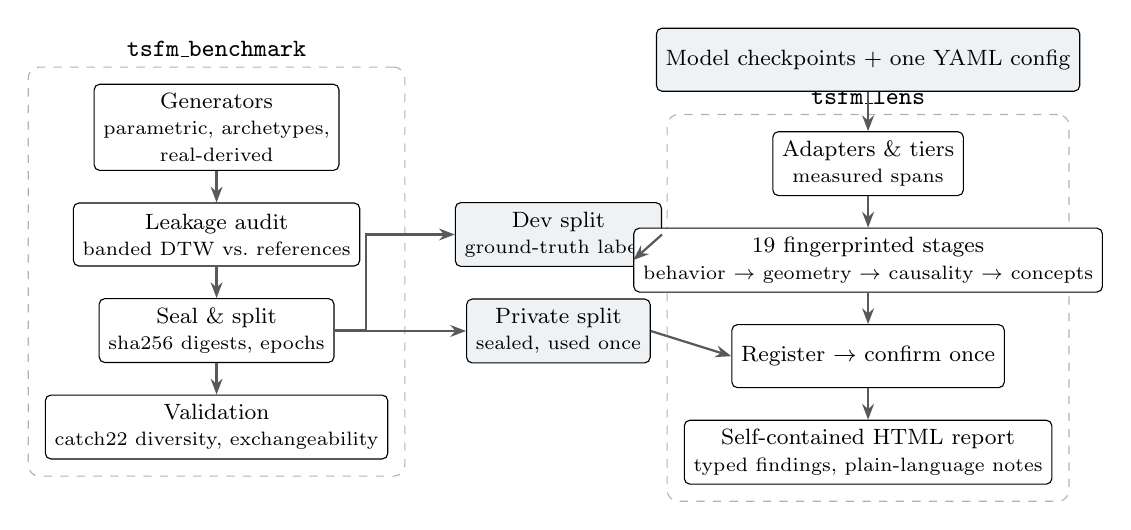
\begin{tikzpicture}[
  node distance=4mm and 6mm,
  box/.style={draw, rounded corners=2pt, align=center, font=\footnotesize, minimum height=8mm, fill=white},
  pkg/.style={draw=gray!60, dashed, rounded corners=4pt, inner sep=6pt},
  lab/.style={font=\scriptsize\itshape, text=gray!70!black},
  arr/.style={-{Stealth[length=2mm]}, thick, gray!70!black}]
  % benchmark package
  \node[box] (gen) {Generators\\{\scriptsize parametric, archetypes,}\\{\scriptsize real-derived}};
  \node[box, below=of gen] (aud) {Leakage audit\\{\scriptsize banded DTW vs.\ references}};
  \node[box, below=of aud] (seal) {Seal \& split\\{\scriptsize sha256 digests, epochs}};
  \node[box, below=of seal] (val) {Validation\\{\scriptsize catch22 diversity, exchangeability}};
  \draw[arr] (gen) -- (aud); \draw[arr] (aud) -- (seal); \draw[arr] (seal) -- (val);
  \begin{scope}[on background layer]
    \node[pkg, fit=(gen)(val), label={[font=\small\bfseries]above:\texttt{tsfm\_benchmark}}] (bp) {};
  \end{scope}
  % corpora
  \node[box, right=12mm of aud, fill=soft] (dev) {Dev split\\{\scriptsize ground-truth labels}};
  \node[box, below=of dev, fill=soft] (priv) {Private split\\{\scriptsize sealed, used once}};
  \draw[arr] (seal.east) -- ++(4mm,0) |- (dev.west);
  \draw[arr] (seal.east) -- ++(4mm,0) |- (priv.west);
  % lens package
  \node[box, right=14mm of dev, yshift=9mm] (ad) {Adapters \& tiers\\{\scriptsize measured spans}};
  \node[box, below=of ad] (st) {19 fingerprinted stages\\{\scriptsize behavior $\to$ geometry $\to$ causality $\to$ concepts}};
  \node[box, below=of st] (reg) {Register $\to$ confirm once};
  \node[box, below=of reg] (rep) {Self-contained HTML report\\{\scriptsize typed findings, plain-language notes}};
  \draw[arr] (ad) -- (st); \draw[arr] (st) -- (reg); \draw[arr] (reg) -- (rep);
  \begin{scope}[on background layer]
    \node[pkg, fit=(ad)(rep), label={[font=\small\bfseries]above:\texttt{tsfm\_lens}}] (lp) {};
  \end{scope}
  \draw[arr] (dev.east) -- (st.west);
  \draw[arr] (priv.east) -- (reg.west);
  \node[box, above=5mm of ad, fill=soft] (ck) {Model checkpoints + one YAML config};
  \draw[arr] (ck) -- (ad);
\end{tikzpicture}
\caption{System overview. \texttt{tsfm\_benchmark} produces leakage-audited, sealed corpora with
exact generative ground truth; \texttt{tsfm\_lens} takes a configuration naming model checkpoints
and produces one report. Dev-split findings are exploratory; the private split is opened once, by
the \texttt{confirm} stage, for claims registered in advance. The two packages install separately
because their dependencies barely overlap.}
\label{fig:overview}
\end{figure}

\section{Related Work}
\label{sec:related}

\paragraph{TSFMs.} TimesFM \citep{das2024timesfm} is decoder-only over 32-step patches; Chronos
\citep{ansari2024chronos} quantizes values and trains a T5 encoder--decoder \citep{raffel2020t5} with a
sampled decoder; Chronos-Bolt uses a direct patch head, and Chronos-2 \citep{ansari2025chronos2} is an
encoder with cross-series group attention; Sundial \citep{liu2025sundial} samples from a flow-matching head
\citep{lipman2023flow}; Timer \citep{liu2024timer} uses 96-step tokens and Lag-Llama \citep{rasul2023lagllama}
reads lagged values. Most normalize each series internally \citep{kim2022revin}, a detail that matters when an
adapter calls a model below its public API (Section~\ref{sec:controls}). \citet{wan2026collapse} document
flat ``collapsed'' forecasts on weakly predictable targets, which we also measure (\fid{PM-07}).

\paragraph{Interpreting time-series models.} Saliency methods for time-series classifiers are unreliable
across architectures \citep{ismail2020benchmarking}; \citet{kalnare2025mechts} apply patching and SAEs to
time-series classifiers. For TSFMs, \citet{wilinski2025exploring} study representational redundancy and
concept steering, and four recent studies train SAEs on one TSFM \citep{mishra2026dissecting,
oublal2026timesae,divo2026zeitgeist,yildirim2026superposition}. Each examines one model or one method. None
compares architectures on a common time axis, validates probes against generative ground truth, separates
input agreement from effect agreement, or tests findings on held-out data.

\paragraph{Methods, tooling and validity.} Probes need control tasks \citep{hewitt2019control,
belinkov2022probing}; patching is sensitive to metrics and corruptions \citep{zhang2024patching,
heimersheim2024patching} and can create illusions \citep{makelov2024illusion}; attention weights are not
explanations \citep{jain2019attention}; saliency maps can fail sanity checks \citep{adebayo2018sanity}. SAE
features vary across seeds \citep{paulo2025seeds}, and crosscoders learn features jointly across models
\citep{lindsey2024crosscoders}. Representation similarity \citep{raghu2017svcca,kornblith2019cka,
bansal2021stitching} underlies claims of convergence \citep{li2016convergent,huh2024platonic}. Libraries such
as TransformerLens, nnsight \citep{fiottokaufman2025nnsight}, pyvene, SAELens \citep{bloom2024saelens} and
Captum \citep{kokhlikyan2020captum} provide primitives for one model; they do not provide comparative
designs, nulls, multiplicity control or confirmation (Table~\ref{tab:tools}). From empirical science we
import pre-registration \citep{nosek2018preregistration}, protection against adaptive reuse of holdouts
\citep{dwork2015reusable}, leakage auditing \citep{kapoor2023leakage} and resampling at the level of the
independent unit \citep{efron1993bootstrap,cameron2008cluster}.

\begin{table}[t]
\centering
\footnotesize
\setlength{\tabcolsep}{3.2pt}
\begin{tabularx}{\textwidth}{@{}Xcccccc@{}}
\toprule
Capability & \rotatebox{70}{TransformerLens} & \rotatebox{70}{nnsight / pyvene} & \rotatebox{70}{SAELens} & \rotatebox{70}{Captum} & \rotatebox{70}{TSFM SAE studies$^{\dagger}$} & \rotatebox{70}{\textbf{\tool{}}} \\
\midrule
Hooks, caching, activation patching                         & \cmark & \cmark & \pmark & \pmark & \pmark & \cmark \\
Sparse dictionaries and feature ablation                     & \pmark & \pmark & \cmark & \xmark & \cmark & \cmark \\
Time-series models without per-model engineering             & \xmark & \pmark & \xmark & \pmark & \xmark & \cmark \\
Measured token$\to$time alignment across architectures       & \xmark & \xmark & \xmark & \xmark & \xmark & \cmark \\
Benchmark with exact generative ground truth, leakage audit  & \xmark & \xmark & \xmark & \xmark & \pmark & \cmark \\
Random-direction nulls and reach controls for every ablation & \xmark & \xmark & \xmark & \xmark & \xmark & \cmark \\
Cross-model concept matching (inputs vs.\ effects)            & \xmark & \xmark & \xmark & \xmark & \xmark & \cmark \\
Series-level resampling and multiplicity ledger              & \xmark & \xmark & \xmark & \xmark & \xmark & \cmark \\
Registered, one-shot confirmation on sealed data             & \xmark & \xmark & \xmark & \xmark & \xmark & \cmark \\
Typed evidence class and generated caveat per claim           & \xmark & \xmark & \xmark & \xmark & \xmark & \cmark \\
One-command report designed for non-experts                  & \xmark & \xmark & \pmark & \xmark & \xmark & \cmark \\
\bottomrule
\end{tabularx}
\caption{Capabilities for comparative TSFM interpretability. \cmark{} provided; \pmark{} possible with user
code or partial; \xmark{} not provided. General libraries are single-model microscopes and complementary
to \tool{}, which uses the same primitives. $^{\dagger}$\citet{mishra2026dissecting,oublal2026timesae,
divo2026zeitgeist,yildirim2026superposition}, judged from the papers.}
\label{tab:tools}
\end{table}

\section{Design Principles}
\label{sec:principles}

\tool{} is opinionated. Each principle below corresponds to a failure that actually happened during
development; Section~\ref{sec:controls} lists them with their numbers. The principles are enforced in
code (as gates, refusals and tests) rather than left as recommendations in documentation.

\begin{description}[leftmargin=1.2em,font=\normalfont\bfseries]
\item[P1. Ground truth by construction.] Every probe is first validated on a case whose answer is
  known. The benchmark records every generative component of every synthetic series (trend order and
  scale, seasonal periods, AR coefficients, changepoints, anomalies, intermittency), so ``does the model
  represent seasonality?'' can be checked against the truth before it is asked of real data. Every
  controlled perturbation (detrending, deseasonalizing, level shifts and six others) is applied to
  series whose components are known, so its effect on the input is known as well.
\item[P2. Alignment is measured, not declared.] A token's time span is measured from the model's own
  impulse response and checked against what the adapter declares. Cross-model analysis happens only
  on a common window axis (Section~\ref{sec:alignment}). A model whose tokens are not time-localized is
  routed to behavioral analysis only, with the verdict rendered in the report.
\item[P3. A causal claim needs a null, a reach control and a same-seed baseline.] Every intervention
  is compared with a random intervention of matched size on the \emph{same} series. Before any
  intervention is trusted, patching a layer into itself must change the forecast by exactly $0.0$,
  and patching in a different layer's activations must change it by a nonzero amount. Sampled models
  are seeded identically in every pair of compared calls.
\item[P4. The series is the unit of inference.] Windows within a series are not independent. All
  confidence intervals and $p$-values resample series (paired, cluster or validation-series
  bootstraps), all $p$-values are floored at $1/n_{\text{boot}}$, and every correction family's
  attainable minimum is checked against its threshold.
\item[P5. Explore, then confirm once.] Everything computed on the dev split is exploratory.
  Hypotheses are frozen with the content hash of the artifact they came from, and the sealed private
  split is opened once. A second look is recorded as a repeated look, and a fresh epoch must be minted
  to confirm again.
\item[P6. Every claim is typed, and failures are loud.] Each finding carries an evidence class
  (\ev{behavioral}, \ev{descriptive}, \ev{geometric}, \ev{linear-translatable},
  \ev{causal within-model}, \ev{illustrative}, \ev{held-out confirmed}) and a caveat generated from
  that class. An unsupported capability is skipped with a reason rendered in the report. An
  unresolvable slice disables the analysis rather than guessing, and a broken assumption raises.
\item[P7. Accessible by default.] The deliverable is one self-contained HTML file that a person with no
  interpretability background can read. Every figure has a caption and a ``What does this mean?''
  explainer that states the figure's purpose, how to read it and its limitations. The headline
  scorecard is computed from artifacts by a pure function; no verdict in it is written by hand.
\end{description}

Two further engineering rules protect reproducibility. New behavior is opt-in, so that sealed corpora
regenerate bit-exactly (golden hashes are pinned in the benchmark tests). And every stage's
configuration is fingerprinted, so a cached artifact computed under a different configuration is
refused rather than silently reused.

\section{System Architecture}
\label{sec:architecture}

\subsection{Repository layout}
\label{sec:layout}

The repository (Figure~\ref{fig:layout}) contains two separately installable packages and a
published example run. The \texttt{main} branch is the clean, publishable surface. A \texttt{dev}
branch preserves the full research history: the research log from which \repo{FINDINGS.md} is
curated, standalone study drivers and experiment configurations that reproduce individual findings.

\begin{figure}[t]
\centering
\footnotesize
\begin{minipage}{0.94\textwidth}
\renewcommand*\DTstyle{\footnotesize\ttfamily}
\renewcommand*\DTstylecomment{\footnotesize\rmfamily\itshape\color{gray!60!black}}
\setlength{\DTbaselineskip}{11pt}
\dirtree{%
.1 TSFM-Interp/.
.2 README.md, FINDINGS.md, DEPENDENCIES.md, CONTRIBUTING.md, CITATION.cff.
.2 tsfm\_benchmark/\DTcomment{corpus generation and validation (installable package)}.
.3 build\_pipeline/\DTcomment{generators, leakage audit, sealing, corruptions, counterfactuals}.
.3 benchmark\_validation/\DTcomment{catch22 diversity, redundancy matching, split exchangeability}.
.3 configs/, example\_runs/, tests/\DTcomment{golden-hash regeneration tests}.
.2 tsfm\_lens/\DTcomment{model analysis (installable package)}.
.3 run.py, configs/examples/, docs/, tests/\DTcomment{CLI, presets, adapters guide, 171 test modules}.
.3 tsfm\_lens/.
.4 models/\DTcomment{adapters, derived tiers, conformance, generic\_hf, template}.
.4 extraction/\DTcomment{hooks, span discovery, alignment gate, zarr store}.
.4 analysis/\DTcomment{L0--L3, lens, attention, statistics, register/confirm}.
.4 sae/\DTcomment{TopK SAE, ablation battery, atlas, transfer, shared-input agreement}.
.4 report/\DTcomment{section builders, derived scorecard, findings, sanitizer}.
.4 pipeline.py, manifest.py, config.py\DTcomment{stages, gates, fingerprints}.
.2 examples/concept\_atlas\_v2/\DTcomment{report.html, config.yaml, run/ (per-stage artifacts)}.
.2 paper/\DTcomment{this paper; figures/make\_figures.py regenerates every data figure}.
}
\end{minipage}
\caption{Repository layout of the \texttt{main} branch. The benchmark and analysis packages are
independent; the example run folder contains every lightweight artifact of the run analyzed in
Section~\ref{sec:casestudy}, so its report and this paper's figures can be regenerated without GPUs.}
\label{fig:layout}
\end{figure}

\subsection{Controlled benchmark generation}
\label{sec:benchmark}

\paragraph{Two leakage tiers.} Real data enter the benchmark only as leakage references, as realism
calibration and as raw material for explicitly labeled generators. The \emph{synthetic} tier touches
no real data and has exact ground truth: the \texttt{parametric} generator is additive (trend,
multiple seasonalities, AR noise, changepoints, anomalies, random walk, intermittency and
heteroskedasticity), and \texttt{random\_parametric} draws a recipe from one of eight frozen
archetypes (trend-dominant, seasonal-dominant, multi-seasonal, regime-switching, AR colored noise,
anomaly-heavy, clean low-noise, noisy chaotic), with four more available opt-in. The
\emph{real-derived} tier (\texttt{mixture}, \texttt{block\_bootstrap} \citep{kunsch1989block} and
\texttt{sequential\_par}) inherits its source distribution, and its ground truth is attributional (which
source, which blocks). Every sample is labeled with its tier. Mixing the tiers in one corpus is a
deliberate design decision: ``no leakage'' and ``realistic'' pull in opposite directions, and the
labels let each analysis report its results per tier rather than choosing one of the two.

\paragraph{Leakage audit and sealing.} Every candidate sample passes a two-stage leakage gate against
real reference collections (the Monash archive \citep{godahewa2021monash}): a cheap prefilter,
then banded dynamic time warping \citep{sakoe1978dtw}. It must also pass a cross-split near-duplicate
check. Dev and private splits draw from disjoint seed ranges; seeds are mixed with SHA-256 (never a
process-salted hash), and every sample is hashed so that \texttt{load\_sealed(verify=True)} detects
tampering. Fresh private \emph{epochs} are minted by striding the seed space, so a consumed private
split can be replaced without touching the dev split.

\paragraph{Validation.} A separate package checks that a corpus is diverse and non-redundant.
Redundancy is measured by shape matching (cross-correlation or DTW). Diversity is measured in the
catch22 feature space \citep{lubba2019catch22}, never on a 2-D embedding, using the participation-ratio
effective dimension \citep{gao2017pr}, nearest-neighbor tails and near-collision rates overall and per
group. Split exchangeability, on which the confirmatory design depends, is tested with an energy
distance \citep{szekely2013energy} plus per-feature TOST equivalence \citep{schuirmann1987tost}, with a
three-state verdict. On the v1 benchmark, dev and private are exchangeable (energy $p=0.51$; 21 of 22
features equivalent; \fid{MP-09}).

\paragraph{Controlled perturbations.} Two perturbation families are built in. Nine structured
\emph{corruptions} (noise, detrend, deseasonalize, frequency shift, level shift, spike, smooth, warp,
dropout) drive the L3 sensitivity and patching analyses; because the underlying components are known,
their effect on the input is known exactly. \emph{Generator counterfactuals} regenerate a series with
one generative knob moved along a dose ladder while every random draw stays fixed; dose~1.0 must
reproduce the original bit-exactly, a free identity test that caught a real bug (\fid{BM-05}).

\subsection{Model adapters and capability tiers}
\label{sec:adapters}

A model enters the system through an adapter (\repo{tsfm_lens/tsfm_lens/models/base.py}) that exposes
\texttt{load}, \texttt{predict} (point forecast plus requested quantiles, in the original scale), the
underlying module, input preparation, a forward pass and \texttt{token\_time\_spans} (one contiguous
time interval per token). Optional methods expose attention and MLP modules and attention patterns.
The adapter's \emph{capability tier} is derived from which methods a subclass actually overrides, never
declared: tier~0 (black box: load and predict), tier~1 (observable: hidden states with spans), tier~2
(steerable: single-pass context, so patching is possible) and tier~3 (decomposable: attention internals).
A stage that needs a higher tier than a model has is skipped for that model, and the report names the
missing method. A \emph{missing capability} raises \texttt{CapabilityUnavailable}, a fact about the
adapter; a \emph{measured} failure of time localization raises \texttt{NotTimeLocalized}, a fact about the
model, and routes it to behavioral analysis only.

Adding a model takes one of three routes. The zero-code \texttt{generic\_hf} adapter discovers layers
and measures spans for a Hugging Face checkpoint and refuses rather than guesses. It has been verified
on Timer, which it recovers with 96-step spans from measurement alone (\fid{MP-01}). A hand-written
adapter is a copy of \repo{tsfm_lens/tsfm_lens/models/TEMPLATE_adapter.py} placed in
\texttt{models/contrib/}, where it is discovered by an AST scan. In either case
\texttt{run.py -{}-check-adapter} runs a one-command checklist: patch-identity and patch-reach
conformance, the alignment gate, span discovery and capability rows. The adapters guide
(\repo{tsfm_lens/docs/ADDING_A_MODEL.md}) documents the pitfalls we encountered, including a worked
account of an adapter that silently bypassed the checkpoint's input normalization (Appendix~\ref{app:adapters}).
Table~\ref{tab:models} lists the models used in this paper.

\begin{table}[t]
\centering
\footnotesize
\setlength{\tabcolsep}{4pt}
\resizebox{\textwidth}{!}{%
\begin{tabular}{@{}lllcccrr@{}}
\toprule
Model & Checkpoint & Architecture & Token & Head & Tier & Params & FLOPs obs. \\
\midrule
\textcolor{tfm}{TimesFM 2.5} & \texttt{google/timesfm-2.5-200m} & decoder-only & 32 & deterministic & 3 & 231M & 42.5\% \\
\textcolor{ctwo}{Chronos-2} & \texttt{amazon/chronos-2} & encoder (+group attn.) & 16 & deterministic & 3 & 119M & 97.5\% \\
\textcolor{sun}{Sundial} & \texttt{thuml/sundial-base-128m} & decoder + flow head & 16 & sampled & 2 & 128M & 22.4\% \\
\textcolor{bolt}{Chronos-Bolt} & \texttt{amazon/chronos-bolt-small} & encoder + patch head & 16 & deterministic & 2 & 48M & 79.3\% \\
\midrule
Chronos-T5 & \texttt{amazon/chronos-t5-*} & encoder--decoder & 1 & sampled & 3 & 8M--709M & 14.4\%$^{a}$ \\
Timer & \texttt{thuml/timer-base-84m} & decoder-only & 96 & deterministic & 2$^{b}$ & 84M & -- \\
Lag-Llama & \texttt{Lag-Llama} & decoder over lags & lags & sampled & 2 & -- & -- \\
\bottomrule
\end{tabular}}
\caption{Models with adapters. The first four form the case study of Section~\ref{sec:casestudy}.
``Token'' is the number of time steps per input token; ``FLOPs obs.''\ is the share of a full
forecast's FLOPs spent in captured blocks, measured with PyTorch's FLOP counter
(\texttt{budget/model\_budget.json}). Sundial's share is low because its sampled flow-matching head runs
outside the captured pass. $^{a}$Chronos-T5-Base; only the encoder is captured, so the sampled decoder
is never observed (\fid{DE-05}). $^{b}$Via the zero-code \texttt{generic\_hf} adapter.}
\label{tab:models}
\end{table}

\subsection{Time alignment across architectures}
\label{sec:alignment}

Cross-model analysis needs a common index. \tool{} measures each token's span from its impulse
response (\texttt{extraction/span\_discovery.py}): a perturbation injected at one time step should move
the tokens whose spans contain it, and the resulting profile is gated on peak-to-pedestal contrast and
contiguity. Given spans $I_j=[s_j,e_j)$ for tokens $j=1,\dots,n$ and windows
$W_w=[wL,(w+1)L)$ of width $L$ (32 by default), the overlap-pooling matrix is
\begin{equation}
  P_{wj} \;=\; \frac{|I_j \cap W_w|}{\sum_{j'} |I_{j'} \cap W_w|},
  \qquad \tilde h_w \;=\; \sum_j P_{wj}\, h_j ,
  \label{eq:pooling}
\end{equation}
and every cross-model analysis runs on the resulting $[\text{series},\text{window},\text{dim}]$ tensors
(Figure~\ref{fig:alignment}). A window that receives no token raises an error rather than producing a
zero row. During extraction an \emph{alignment gate} injects an impulse into each window and checks,
layer by layer, that the matching pooled window moves most. Because coarse tokens cannot resolve fine
windows (a 96-step token on 32-step windows can reach at most one third of diagonal hits), the gate
normalizes hits by their attainable ceiling (\fid{MP-02}). The impulse amplitude is self-calibrated per
checkpoint and context length.

\begin{figure}[t]
\centering
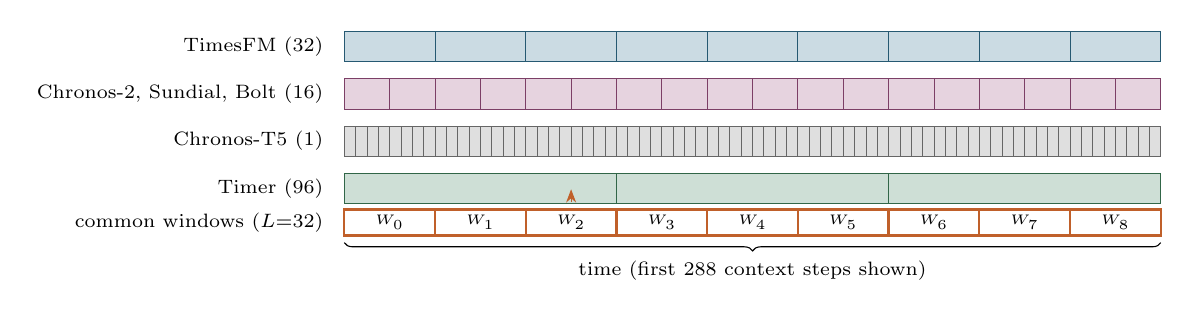
\begin{tikzpicture}[x=0.36mm,y=6mm,font=\scriptsize]
  \foreach \row/\name/\w/\col in {3/TimesFM (32)/32/tfm, 2/{Chronos-2, Sundial, Bolt (16)}/16/ctwo, 1/Chronos-T5 (1)/4/gray, 0/Timer (96)/96/sun}{
    \node[anchor=east] at (-4,\row) {\name};
    \pgfmathtruncatemacro{\n}{288/\w-1}
    \foreach \k in {0,...,\n}{
      \draw[fill=\col!25, draw=\col!80!black, line width=0.3pt] (\k*\w,\row-0.32) rectangle ({(\k+1)*\w},\row+0.32);
    }
  }
  \foreach \k in {0,...,8}{
    \draw[thick, accent] (\k*32,-1.0) rectangle ({(\k+1)*32},-0.45);
    \node[font=\tiny] at (\k*32+16,-0.72) {$W_{\k}$};
  }
  \node[anchor=east] at (-4,-0.72) {common windows ($L{=}32$)};
  \draw[-{Stealth}, accent] (80,-0.3) -- (80,-0.02);
  \draw[decorate,decoration={brace,amplitude=3pt,mirror}] (0,-1.15) -- (288,-1.15) node[midway,below=3pt] {time (first 288 context steps shown)};
\end{tikzpicture}
\caption{Architecture-agnostic time alignment. Tokens of each model cover measured, contiguous spans
of different widths (Chronos-T5's one-step tokens are drawn in groups of four); Equation~\eqref{eq:pooling}
pools them by overlap onto common windows, so that all cross-model statistics compare the same stretch of
time.}
\label{fig:alignment}
\end{figure}

\subsection{The stage pipeline and its gates}
\label{sec:stages}

An analysis is a directed pipeline of 19 stages (Figure~\ref{fig:stages}), each writing typed artifacts
into the run directory. Stages skip themselves when their artifacts exist, and each stage declares the
configuration keys its artifacts depend on. These are fingerprinted, so a changed setting marks exactly
the dependent artifacts stale and a stale artifact is refused. Three gates decide what runs and write
their decisions to JSON, so the report can name them as skip reasons: the \emph{tier gate} (does every
model support this stage?), the \emph{run-shape gate} (comparison-only stages are dropped for a single
model) and the \emph{routing gate} (models that are not time-localized receive behavioral analysis
only). Extraction captures the residual stream into a chunked zarr store in float16 and runs the
alignment gate. All interventions go through a single primitive (\texttt{hooks.token\_patch}), which
raises if the model silently splits a batch.

\begin{figure}[t]
\centering
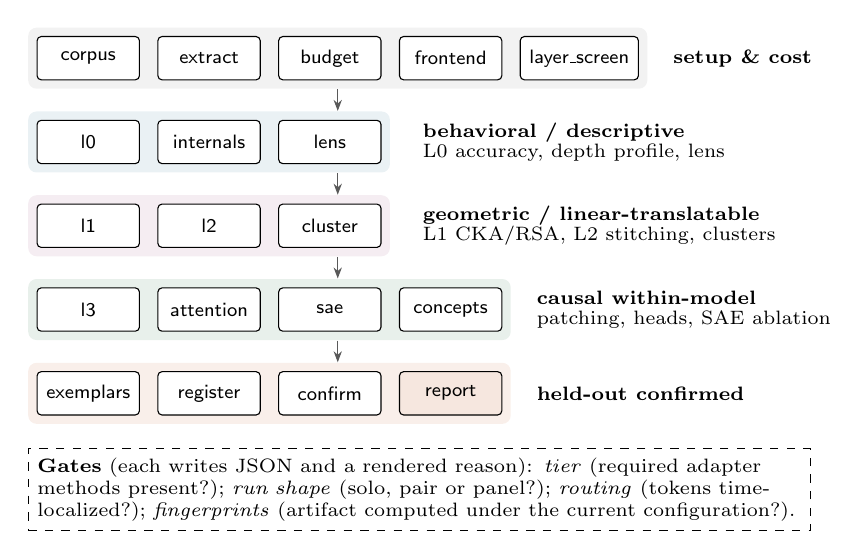
\begin{tikzpicture}[
  node distance=2.2mm and 2.2mm,
  st/.style={draw, rounded corners=1.5pt, font=\scriptsize\sffamily, minimum width=13mm, minimum height=5.5mm, fill=white},
  arr/.style={-{Stealth[length=1.4mm]}, gray!70!black},
  band/.style={rounded corners=3pt, inner sep=3pt},
  blab/.style={font=\scriptsize\bfseries, anchor=west}]
  \node[st] (corpus) {corpus};
  \node[st, right=of corpus] (extract) {extract};
  \node[st, right=of extract] (budget) {budget};
  \node[st, right=of budget] (frontend) {frontend};
  \node[st, right=of frontend] (screen) {layer\_screen};
  \node[st, below=5mm of corpus] (l0) {l0};
  \node[st, right=of l0] (internals) {internals};
  \node[st, right=of internals] (lens) {lens};
  \node[st, below=5mm of l0] (l1) {l1};
  \node[st, right=of l1] (l2) {l2};
  \node[st, right=of l2] (cluster) {cluster};
  \node[st, below=5mm of l1] (l3) {l3};
  \node[st, right=of l3] (attention) {attention};
  \node[st, right=of attention] (sae) {sae};
  \node[st, right=of sae] (concepts) {concepts};
  \node[st, below=5mm of l3] (exemplars) {exemplars};
  \node[st, right=of exemplars] (register) {register};
  \node[st, right=of register] (confirm) {confirm};
  \node[st, right=of confirm, fill=accent!15] (report) {report};
  \begin{scope}[on background layer]
    \node[band, fill=gray!10, fit=(corpus)(screen)] (b1) {};
    \node[band, fill=tfm!10, fit=(l0)(lens)] (b2) {};
    \node[band, fill=ctwo!10, fit=(l1)(cluster)] (b3) {};
    \node[band, fill=sun!12, fit=(l3)(concepts)] (b4) {};
    \node[band, fill=accent!10, fit=(exemplars)(report)] (b5) {};
  \end{scope}
  \node[blab] at ($(b1.east)+(2mm,0)$) {setup \& cost};
  \node[blab, align=left] at ($(lens.east)+(4mm,0)$) {behavioral / descriptive\\[-1pt]{\scriptsize\rmfamily\mdseries L0 accuracy, depth profile, lens}};
  \node[blab, align=left] at ($(cluster.east)+(4mm,0)$) {geometric / linear-translatable\\[-1pt]{\scriptsize\rmfamily\mdseries L1 CKA/RSA, L2 stitching, clusters}};
  \node[blab, align=left] at ($(b4.east)+(2mm,0)$) {causal within-model\\[-1pt]{\scriptsize\rmfamily\mdseries patching, heads, SAE ablation}};
  \node[blab, align=left] at ($(b5.east)+(2mm,0)$) {held-out confirmed};
  \draw[arr] (b1.south) -- (b2.north -| b1.south);
  \draw[arr] (b2.south -| b1.south) -- (b3.north -| b1.south);
  \draw[arr] (b3.south -| b1.south) -- (b4.north -| b1.south);
  \draw[arr] (b4.south -| b1.south) -- (b5.north -| b1.south);
  % gates
  \node[draw, dashed, font=\scriptsize, align=left, anchor=north west, text width=0.8\textwidth, fill=white] at ($(b5.south west)+(0,-3mm)$)
    {\textbf{Gates} (each writes JSON and a rendered reason): \emph{tier} (required adapter methods present?);
     \emph{run shape} (solo, pair or panel?); \emph{routing} (tokens time-localized?);
     \emph{fingerprints} (artifact computed under the current configuration?).};
\end{tikzpicture}
\caption{The 19-stage pipeline, grouped by the strongest evidence class each group can produce.
Stages below a gate that cannot run for a model are skipped for that model with the reason rendered in
the report. Only \texttt{confirm}, on the sealed private split, produces \ev{held-out confirmed}
evidence.}
\label{fig:stages}
\end{figure}

\subsection{The report: interpretability for non-specialists}
\label{sec:report}

The deliverable of a run is a single HTML file with no external dependencies
(\repo{examples/concept_atlas_v2/report.html}; Appendix~\ref{app:report} shows excerpts). It is designed
so that a reader with no background in interpretability can follow it, and so that an expert can audit
every number.

\begin{itemize}
  \item \textbf{Question-first structure.} After an ``at a glance'' block, seven parts pose plain
    questions (``Is the comparison fair?'', ``How well does each model forecast?'', ``Where does the
    forecast form?'', ``Do the models represent things the same way?'', ``What causally drives the
    forecast?'', ``Features and concepts'', ``Robustness and held-out confirmation''), and each stage
    section opens with a card stating its question, its method, what a good and a bad result look like,
    and what it cannot tell you.
  \item \textbf{Every figure explained.} Each figure has a caption plus a collapsible ``What does this
    mean?'' note giving its purpose, how to read it and its limitations; the example report contains
    361 such notes across its 19 sections. A glossary, a methods appendix and a gallery of known failure
    modes are generated from the code.
  \item \textbf{Derived, auditable verdicts.} The scorecard (33 rows in the example) is produced by a
    pure reduction over artifacts with no model names hard-coded: each row shows the measured value, the
    reference it is compared with (a null, a floor, a ceiling or a baseline) and the rule that turns the
    two into a verdict, so a reader can apply a different rule to the same numbers. A missing reference
    renders as ``not comparable''.
  \item \textbf{Typed findings.} Every claim is a \texttt{Finding} record with an identifier, stage,
    evidence class, technical text, a plain-language sentence and a caveat generated from the evidence
    class. The example run emits 126 findings (58 descriptive, 29 behavioral, 21 causal within-model,
    12 linear-translatable, 4 geometric, 2 illustrative), serialized to \texttt{report/findings.json}.
  \item \textbf{Nothing silently missing.} A stage that did not run renders as ``not run'' with its gate
    reason; a stage that raised renders as a visible ``section failed''. A multiplicity ledger lists every
    correction family (45 families and 3{,}599 comparisons in the example) and flags any family whose
    smallest attainable adjusted $p$-value cannot reach $\alpha$.
  \item \textbf{Reading levels.} A toggle switches between a headline view (fairness card, accuracy and
    confirmed findings only), the standard view and a methods view with every detail expanded.
\end{itemize}

\noindent The complete analysis is one command:
\begin{center}
\texttt{python run.py -{}-config configs/examples/large\_4model.yaml}
\end{center}
and smaller presets cover a CPU-only smoke test with mock models, a single real model and a pair
(\repo{tsfm_lens/configs/README.md}).

\section{Measurement Methods}
\label{sec:methods}

This section defines what each stage measures. Throughout, $x\in\mathbb{R}^{T}$ is a context of length
$T$ (512 in the case study), $y\in\mathbb{R}^{H}$ the true continuation ($H=64$), $\hat y$ a model's point
forecast and $h^{(\ell)}$ the residual stream after block $\ell$.

\subsection{Behavior and cost (L0)}
\label{sec:l0}

Accuracy is scored per series with MASE \citep{hyndman2006mase},
\begin{equation}
  \mathrm{MASE}(\hat y, y) \;=\; \frac{\tfrac1H\sum_{t=1}^{H}|y_t-\hat y_t|}
       {\max\!\big(\tfrac{1}{T-m}\sum_{t=m+1}^{T}|x_t-x_{t-m}|,\;\epsilon_x\big)},
\end{equation}
with the seasonal lag $m$ taken from ground truth where available, and a scale floor $\epsilon_x$
because on intermittent series the naive denominator collapses and MASE spuriously improves
(\fid{MN-23}). sMAPE, pinball loss \citep{gneiting2007scoring} and interval calibration are reported
alongside. Model pairs are compared with a paired bootstrap over series, per family and overall, with
Holm correction across all pairs and families \citep{holm1979}. Each model's repeat-run \emph{noise floor}
(two identical runs with different seeds) is measured so that a difference can be read in floor units;
a deterministic model has a floor of zero, which the report states rather than using as a referee. The
\texttt{budget} stage measures parameters by role, FLOPs with PyTorch's \texttt{FlopCounterMode},
latency, memory and the share of forecast FLOPs spent inside captured blocks (Table~\ref{tab:models}).
The \texttt{frontend} stage tests the tokenizer before any layer runs: scale equivariance (forecasting
$c\,x$ should give $c\,\hat y$), NaN handling and quantization resolution.

\subsection{Geometry and linear translatability (L1, L2)}
\label{sec:l1l2}

For aligned activations $A\in\mathbb{R}^{n\times d_a}$ and $B\in\mathbb{R}^{n\times d_b}$ over the same
$n$ series (mean-pooled over windows, then centered), linear CKA \citep{kornblith2019cka} is
\begin{equation}
  \mathrm{CKA}(A,B) \;=\; \frac{\|B^{\top}A\|_F^2}{\|A^{\top}A\|_F\,\|B^{\top}B\|_F}.
\end{equation}
It is computed for every layer pair of every model pair, with a cluster bootstrap over series and a
shuffled-series null that breaks correspondence while preserving each model's marginal geometry. L2 fits
ridge maps between layers and reports only the \emph{gain} of the stitched prediction over an
input-feature baseline, never a raw $R^2$, because a large part of any layer is linearly predictable from
the input alone. Activation clusterings are compared across models with adjusted mutual information
\citep{vinh2010ami}. These are \ev{geometric} and \ev{linear-translatable} claims; they say nothing about
what the model uses.

\subsection{Perturbation and patching (L3)}
\label{sec:l3}

For each corruption $c$ of the nine in Section~\ref{sec:benchmark}, L3 records a sensitivity
\emph{fingerprint}, the relative activation change $\|h^{(\ell)}(c(x))-h^{(\ell)}(x)\|/\|h^{(\ell)}(x)\|$ per
layer, and a within-model \emph{restoration curve}: the fraction of the forecast damage undone by
patching the clean activations of layer $\ell$ (whole layer, or one window at a time) into the corrupted
forward pass. Two models are compared by rank-correlating their fingerprints on the relative depth range
they share, never by transplanting activations between models. Restoration is \ev{causal within-model};
agreement between models is correlational.

\subsection{Depth: lens, internals and coverage}
\label{sec:depth}

A skip lens decodes the forecast from each layer through the model's own head, and a tuned ridge lens
\citep{belrose2023tuned} fits a per-layer readout; the crystallization depth is the shallowest layer
whose lens forecast is within tolerance of the final one. \texttt{internals} reports per-layer effective
dimension (participation ratio), decodability of benchmark families and CKA to the input.
\texttt{layer\_screen} selects the layers that deserve expensive analysis with a cheap proxy
(\texttt{work\_bend}). Two design points qualify every depth claim. First, the depth axis is the fraction of
the \emph{whole} stack's blocks, including uncaptured parts, so Chronos-T5's last captured encoder block
sits at 0.478 rather than 1.0 (\fid{DE-04}). Second, the lens is withheld for a model whose head reads
positions the patch never writes (\texttt{forecast\_reads\_patched\_positions}), because such a lens returns
a perfectly flat and meaningless curve (\fid{DE-03}).

\subsection{Causal concepts}
\label{sec:concepts}

\paragraph{Sparse dictionaries.} For each target layer, \tool{} trains a TopK sparse autoencoder
\citep{makhzani2013ksparse,gao2025topk} on token-level activations,
\begin{equation}
  z(h) = \operatorname{TopK}\!\big(W_e(h-b_d)+b_e\big),\qquad \hat h = W_d\,z(h) + b_d ,
\end{equation}
with the dictionary size chosen by a search, an auxiliary loss that revives dead atoms and a minimum
number of training steps (\fid{MP-03}). Fidelity, dead rate and forecast preservation are reported per
target. Because a single SAE seed is not reproducible \citep{paulo2025seeds}, $n_{\text{seeds}}$ replicate
dictionaries are trained at the primary's size to measure a within-model reproducibility ceiling
(\fid{MP-04}).

\paragraph{The ablation battery.} A feature $i$ is tested on the $k$ series on which it fires most. For
those series, the layer's activations are replaced by the SAE reconstruction with $z_i$ set to zero, and the
forecast is compared with the forecast under the full reconstruction:
\begin{equation}
  \Delta_i^{(c)}(x) \;=\; g_c\!\big(f(x;\,h^{(\ell)}\!\leftarrow\!\hat h_{-i})\big) - g_c\!\big(f(x;\,h^{(\ell)}\!\leftarrow\!\hat h)\big),
  \label{eq:ablation}
\end{equation}
where $f(x;\,h\!\leftarrow\!\cdot)$ is the forecast with layer $\ell$ patched and $g_c$ is one of nine
forecast \emph{channels}: trend, seasonal strength, spectral centroid, level, dispersion, near- and
far-horizon shape distance, MASE and flatness. Using the full reconstruction, not the clean forecast, as the
baseline keeps the dictionary's own reconstruction error from being charged to the feature. The
\emph{null} removes a random unit direction in code space, scaled to the mean magnitude the ablations
remove, on the \emph{same} series; the feature clears channel $c$ if its mean $|\Delta_i^{(c)}|$ exceeds
the 95th percentile of the null draws restricted to its own rows. The row matching matters: a feature
whose top series happen to sit in a high-response regime would otherwise clear a pooled null on that
alone. The channel vector used downstream is $v_i^{(c)} = \overline{\Delta_i^{(c)}}/q_{95}^{(c)}$, the
signed mean effect in null units. The near- and far-horizon shape channels are distances ($\ge 0$) and are
treated as undirected everywhere, including in generated text. Before any feature is scored, a
\emph{reach probe} requires that patching the layer's own clean activations into itself changes the
forecast by exactly $0.0$ and that patching another layer's activations changes it by a relative amount
above $10^{-3}$ (Figure~\ref{fig:battery}). A target that fails the probe is withheld with its reason,
because a table of zeros from a patch that never lands reads as ``these features do not matter''.

\begin{figure}[t]
\centering
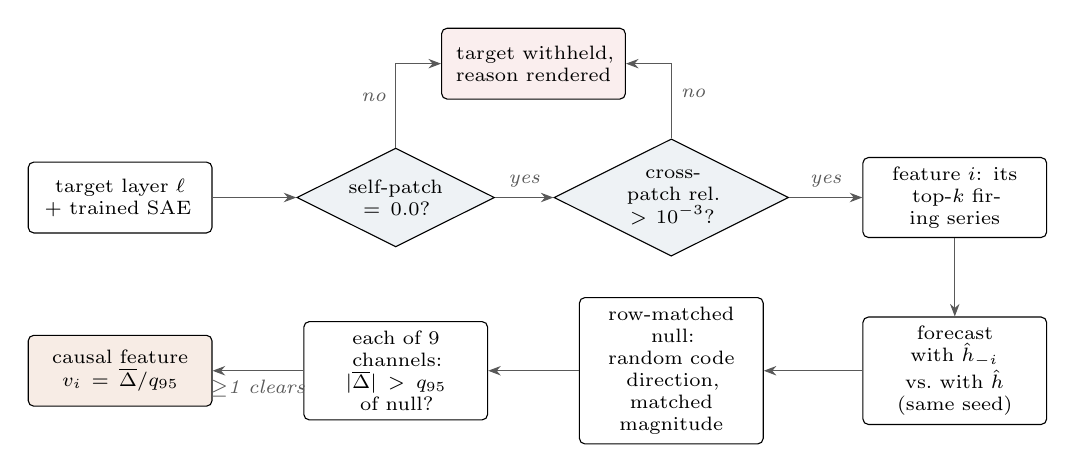
\begin{tikzpicture}[
  box/.style={draw, rounded corners=2pt, align=center, font=\scriptsize, minimum height=9mm, fill=white, text width=21mm},
  gate/.style={draw, diamond, aspect=2.0, align=center, font=\scriptsize, inner sep=0.5pt, fill=soft, text width=15mm},
  arr/.style={-{Stealth[length=1.6mm]}, gray!70!black},
  lab/.style={font=\scriptsize\itshape, text=gray!70!black}]
  \node[box] (tgt) at (0,0) {target layer $\ell$\\+ trained SAE};
  \node[gate] (self) at (3.5,0) {self-patch\\$=0.0$?};
  \node[gate] (cross) at (7.0,0) {cross-patch rel.\\$>10^{-3}$?};
  \node[box] (rows) at (10.6,0) {feature $i$: its\\top-$k$ firing series};
  \node[box, fill=bad!8] (wh) at (5.25,1.7) {target withheld,\\reason rendered};
  \node[box] (abl) at (10.6,-2.2) {forecast with $\hat h_{-i}$\\vs.\ with $\hat h$\\(same seed)};
  \node[box] (null) at (7.0,-2.2) {row-matched null:\\random code direction,\\matched magnitude};
  \node[box] (chan) at (3.5,-2.2) {each of 9 channels:\\$|\overline{\Delta}|>q_{95}$ of null?};
  \node[box, fill=accent!12] (vec) at (0,-2.2) {causal feature\\$v_i=\overline{\Delta}/q_{95}$};
  \draw[arr] (tgt) -- (self);
  \draw[arr] (self) -- node[above,lab]{yes} (cross);
  \draw[arr] (cross) -- node[above,lab]{yes} (rows);
  \draw[arr] (self.north) |- node[left,lab,pos=0.3]{no} (wh.west);
  \draw[arr] (cross.north) |- node[right,lab,pos=0.3]{no} (wh.east);
  \draw[arr] (rows) -- (abl);
  \draw[arr] (abl) -- (null);
  \draw[arr] (null) -- (chan);
  \draw[arr] (chan) -- node[below,lab]{$\ge$1 clears} (vec);
\end{tikzpicture}
\caption{The ablation battery. A target is scored only after both reach controls pass; each feature is
ablated on its own top-firing series and compared, channel by channel, with a random-direction null on
exactly those series. Only features that clear at least one channel enter the concept analyses.}
\label{fig:battery}
\end{figure}

\paragraph{From features to concepts.} Causal features are grouped at three granularities, each
answering a different question. \emph{Per-target concepts} cluster one layer's feature vectors with
$k$-means, choosing $k$ by silhouette \citep{rousseeuw1987silhouette} among values whose smallest cluster
has at least three members; a target with no admissible $k$ is reported as \emph{non-modular}. (Without
the minimum-size constraint, silhouette rewards splitting off a single outlier; \fid{SH-20}.) The
\emph{concept atlas} pools causal features from every model and layer and cuts a complete-linkage
dendrogram at cosine 0.9, which guarantees that every pair of members has cosine at least 0.9; an atlas
concept is a shared \emph{causal-effect profile}, not a shared input. \emph{Families} are a coarser,
readable tiling: average linkage plus nearest-centroid assignment at cosine 0.5, with the number of
families chosen by a parsimony rule and tested against a column-shuffle null. Families are titled
deterministically from their directed channels (Figure~\ref{fig:families}).

\subsection{Two notions of sharing}
\label{sec:sharing}

Whether a concept is ``shared'' between models is two separate questions, and conflating them produces
wrong answers in both directions (Section~\ref{sec:controls}). \tool{} answers them separately and then
combines them in an evidence ladder (Figure~\ref{fig:ladder}).

\paragraph{Same inputs.} \emph{Concept transfer} asks whether some feature in another model separates a
concept's top-$k$ firing series from the rest, scored by AUC, against a null of random series subsets
matched on benchmark strata (family and archetype); the test is run in both directions and a transfer is
\emph{reciprocal} if both legs clear. At atlas scale, $p$-values are corrected by Benjamini--Hochberg
\citep{benjamini1995fdr} per ordered model pair and leg. When concept profiles compare what two concept
parts fire on, input agreement is measured as the overlap of their top-$k$ series (hypergeometric test
with BH), never as a whole-series correlation, because two sparse features can have $\rho=0.80$ with no
shared top series (\fid{MN-19}).

\paragraph{Same effect on the same inputs.} \emph{Shared-input causal agreement} takes every
reciprocal-FDR transfer and ablates the feature (or concept part) on each side on the \emph{same} series
set $U$. Each side must first clear its own random-direction null on $U$ to be scorable. Two statistics,
level concordance and the cosine of the shape effects, must then beat both sides'
\emph{activation-matched random-feature floors}: sets of equally active features whose ablation defines
what agreement looks like by chance. A pair is ``same causal effect'' if both statistics beat both floors,
``level only'' or ``shape only'' if one does, and ``acts differently'' only if a statistic falls below the
floors' 5th percentile; failing to beat the 95th percentile is ``no specific agreement''. The distinction
matters: absence of agreement is not evidence of disagreement (\fid{MN-18}).

\paragraph{Sharing classes.} Each atlas concept then receives a \texttt{sharing\_class}: \emph{shared}
(same effect and same inputs across models), \emph{partially shared}, \emph{convergent} (same effect,
different inputs) or \emph{single-model}. A concept part is flagged provenance-driven when at least 80\% of
its top series come from one real-derived generator.

\begin{figure}[t]
\centering
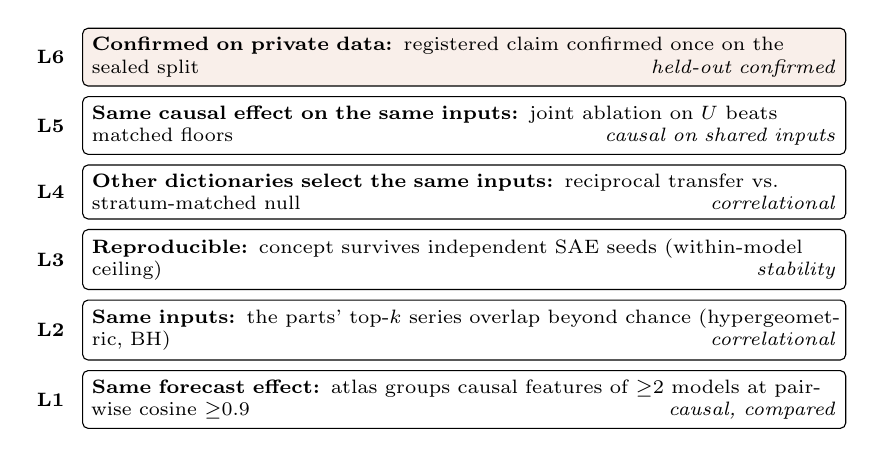
\begin{tikzpicture}[
  rung/.style={draw, rounded corners=2pt, font=\scriptsize, align=left, text width=0.78\textwidth, minimum height=6.5mm, fill=white},
  tag/.style={font=\scriptsize\bfseries, anchor=east},
  arr/.style={-{Stealth[length=1.5mm]}, gray!60!black}]
  \node[rung] (r1) {\textbf{Same forecast effect:} atlas groups causal features of $\ge$2 models at pairwise cosine $\ge$0.9 \hfill \textit{causal, compared}};
  \node[rung, above=1.2mm of r1] (r2) {\textbf{Same inputs:} the parts' top-$k$ series overlap beyond chance (hypergeometric, BH) \hfill \textit{correlational}};
  \node[rung, above=1.2mm of r2] (r3) {\textbf{Reproducible:} concept survives independent SAE seeds (within-model ceiling) \hfill \textit{stability}};
  \node[rung, above=1.2mm of r3] (r4) {\textbf{Other dictionaries select the same inputs:} reciprocal transfer vs.\ stratum-matched null \hfill \textit{correlational}};
  \node[rung, above=1.2mm of r4] (r5) {\textbf{Same causal effect on the same inputs:} joint ablation on $U$ beats matched floors \hfill \textit{causal on shared inputs}};
  \node[rung, above=1.2mm of r5, fill=accent!10] (r6) {\textbf{Confirmed on private data:} registered claim confirmed once on the sealed split \hfill \textit{held-out confirmed}};
  \foreach \i in {1,...,6}{ \node[tag] at ($(r\i.west)+(-1mm,0)$) {L\i}; }
\end{tikzpicture}
\caption{The concept evidence ladder used by the report (computed by \texttt{concept\_verdicts} in \texttt{report/derived.py}).
Every causal feature has already passed the ablation battery (Figure~\ref{fig:battery}). Each rung is a
separate test with its own null, and the report states the highest rung each concept reaches together with
the rule that produced its verdict. ``Shared'' in this paper means the \texttt{shared} sharing class: same
effect (L1) and same inputs (L2).}
\label{fig:ladder}
\end{figure}

\section{Statistical Protocol}
\label{sec:statistics}

A system that runs thousands of comparisons per report must control how often it is fooled. \tool{}
does so with four mechanisms, summarized in Table~\ref{tab:claims}.

\paragraph{The series is the resampling unit.} Windows of one series share its trend, noise process and
scale, so treating them as independent overstates precision. Every interval and $p$-value in \tool{}
resamples whole series \citep{efron1993bootstrap,cameron2008cluster}: a paired bootstrap for accuracy
differences, a cluster bootstrap for CKA, a validation-series interval (probes held fixed) for stitching
and a paired cluster bootstrap for patching. Train/validation splits are also made by series and sampled
by stratum, never by slicing the head of a corpus that is stored grouped by task.

\paragraph{A multiplicity ledger.} Every test is assigned to a named correction family (Holm for
confirmatory families, Benjamini--Hochberg for discovery-oriented atlas transfers). Resampled $p$-values
are floored at $1/n_{\text{boot}}$ \citep{phipson2010permutation}, which means a Holm family of $m$ tests
cannot produce an adjusted $p$ below $m/n_{\text{boot}}$. The ledger computes this attainable minimum
for every family and flags families in which no test could ever be significant, a failure mode that grows
silently as models are added (the number of pairwise comparisons is quadratic). The example run has 45
correction families and 3{,}599 comparisons; its most stringent L0 family (30 tests over 6 model pairs)
has a minimum attainable Holm $p$ of 0.015 at $n_{\text{boot}}=2000$.

\paragraph{Noise floors and power.} Effects are read against reference values that come from the run
itself: repeat-run noise floors for accuracy, shuffled-series nulls for CKA, input-feature baselines for
stitching, random-direction nulls and activation-matched floors for ablations, and replicate-seed
ceilings for SAE reproducibility. Before the private split is opened, the confirm stage computes each
registered claim's minimum detectable effect at the private sample size by simulation (for example, a
$\Delta$MASE of 0.155 at $n=240$ with 80\% power), so that a non-replication can be read as ``absent'' or
``underpowered''.

\paragraph{Register, then confirm once.} The \texttt{register} stage freezes hypotheses drawn from dev
results into a registry, together with the content hash of each dev artifact a hypothesis came from; the
registry itself is hashed. The \texttt{confirm} stage refuses to run if a hash does not match, requires
the private split's seal to verify, tests each claim once and refuses to overwrite its own artifact.
Forcing a rerun is recorded as \texttt{repeated\_look}, and a consumed split is replaced by minting a new
epoch (Figure~\ref{fig:confirm}). This is pre-registration \citep{nosek2018preregistration} applied to a
software pipeline, and a guard against adaptive overfitting of the holdout \citep{dwork2015reusable}.
Findings that were never registered cannot be rescued after the fact.

\begin{figure}[t]
\centering
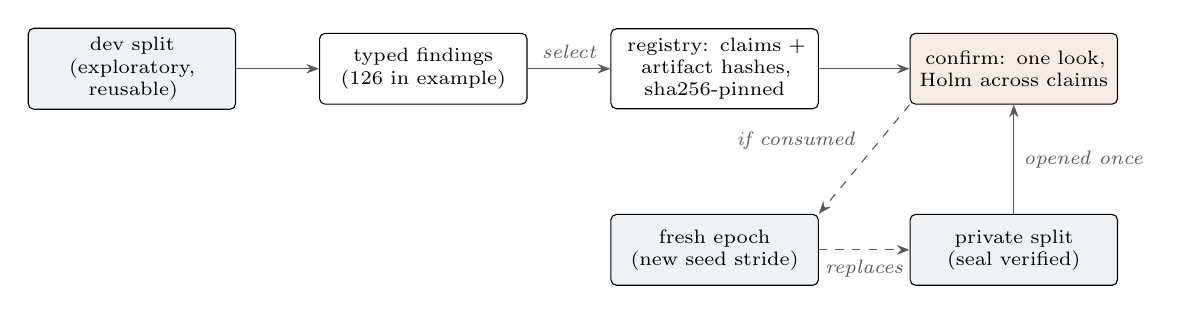
\begin{tikzpicture}[
  box/.style={draw, rounded corners=2pt, align=center, font=\scriptsize, minimum height=9mm, fill=white, text width=24mm},
  arr/.style={-{Stealth[length=1.6mm]}, gray!70!black},
  lab/.style={font=\scriptsize\itshape, text=gray!70!black}]
  \node[box, fill=soft] (dev) at (0,0) {dev split\\(exploratory, reusable)};
  \node[box] (find) at (3.7,0) {typed findings\\(126 in example)};
  \node[box] (reg) at (7.4,0) {registry: claims +\\artifact hashes,\\sha256-pinned};
  \node[box, fill=accent!12] (conf) at (11.2,0) {confirm: one look,\\Holm across claims};
  \node[box, fill=soft] (priv) at (11.2,-2.3) {private split\\(seal verified)};
  \node[box, fill=soft] (epoch) at (7.4,-2.3) {fresh epoch\\(new seed stride)};
  \draw[arr] (dev) -- (find);
  \draw[arr] (find) -- node[above,lab]{select} (reg);
  \draw[arr] (reg) -- (conf);
  \draw[arr] (priv) -- node[right,lab]{opened once} (conf);
  \draw[arr, dashed] (conf.south west) -- node[above left,lab]{if consumed} (epoch.north east);
  \draw[arr, dashed] (epoch) -- node[below,lab]{replaces} (priv);
\end{tikzpicture}
\caption{The confirmatory protocol. Only claims registered before the private split is opened can be
confirmed; a second look is recorded, and replicating again requires a newly minted epoch.}
\label{fig:confirm}
\end{figure}

\begin{table}[t]
\centering
\footnotesize
\setlength{\tabcolsep}{3pt}
\begin{tabularx}{\textwidth}{@{}>{\raggedright}p{2.6cm}>{\raggedright}p{2.7cm}>{\raggedright}X>{\raggedright}p{1.9cm}l@{}}
\toprule
Claim type & Test statistic & Null / reference & Correction & Held-out \\
\midrule
Model A more accurate (per family) & paired $\Delta$MASE, series bootstrap & zero difference; repeat-run noise floor & Holm over all pairs $\times$ families & \cmark \\
Layers share geometry & linear CKA, cluster bootstrap & shuffled-series null at the same layer pair & per model pair & \cmark \\
Layer linearly translatable & ridge stitching gain & input-feature baseline (gain $=0$) & per pair & -- \\
Depth reaction agrees & Spearman $\rho$ of fingerprints on shared depth & bootstrap CI of $\rho$ & per corruption & \cmark \\
Layer restores forecast & restoration fraction & self-patch $=0$, cross-patch $\neq 0$ & per model & -- \\
Feature is causal & mean $|\Delta^{(c)}|$ on own rows & row-matched random-direction $q_{95}$ & per channel (count vs.\ chance) & -- \\
Concept reproducible & best-match cosine across seeds & within-model replicate ceiling & -- & -- \\
Same inputs & top-$k$ AUC in other model & stratum-matched random subsets & BH per ordered pair and leg; Holm when registered & \cmark \\
Same effect on same inputs & level concordance; shape cosine & activation-matched feature-set floors ($q_{95}$ agree, $q_{05}$ differ) & per test & -- \\
Families are real & number and coverage of families & column-shuffle null & -- & -- \\
\bottomrule
\end{tabularx}
\caption{Every claim type the case study reports, the statistic that tests it, the reference it must
beat, its multiplicity correction and whether the \texttt{confirm} stage currently re-tests it on
private data. Claim types without a held-out mark are reported as exploratory.}
\label{tab:claims}
\end{table}

\section{Case Study: Four Time-Series Foundation Models}
\label{sec:casestudy}

\subsection{Setup}
\label{sec:setup}

We analyze TimesFM~2.5, Chronos-2, Sundial and Chronos-Bolt (Table~\ref{tab:models}) with the preset
\repo{tsfm_lens/configs/concept_atlas_v2.yaml}. The dev corpus has 965 series in five generator families
(\texttt{parametric}, \texttt{random\_parametric}, \texttt{mixture}, \texttt{block\_bootstrap},
\texttt{sequential\_par}); the real-derived families draw on Monash weather, ETT \citep{zhou2021informer}
and the Chronos electricity and traffic collections. Contexts are 512 steps, the horizon is 64 and the
alignment window is 32. SAEs are trained on 29 target layers (TimesFM: 10, at stride 2; Chronos-2: 7;
Sundial: 9; Chronos-Bolt: 3), with three replicate seeds each for stability, and $n_{\text{boot}}=2000$
throughout. The private split is 800 sealed series (epoch 0 of the v2 benchmark), opened once. The whole
run took 6.43 hours on a single NVIDIA RTX A5000 (24~GB), of which SAE training took 2.39 hours and the
concept stage 3.72 hours (Appendix~\ref{app:repro}). All artifacts are in
\repodir{examples/concept_atlas_v2/run}; results that come from other runs recorded in the ledger are
marked with their \repo{FINDINGS.md} identifier.

Before turning to the research questions, Table~\ref{tab:character} summarizes the models' behavior,
which later sections use as context. Chronos-2 is the most accurate on the dev corpus and on held-out
data. Sundial covers only 37\% of outcomes with its nominal 80\% interval. TimesFM and Sundial propagate
an injected NaN to the forecast without raising, while the Chronos models handle it. Behind the Sundial
row is a bug found during this work: the first Sundial adapter bypassed the checkpoint's input
normalization, and the \texttt{frontend} stage's scale-equivariance residual (38.43 context standard
deviations, against $\le 0.009$ for the other models) was at first read as a property of the model
(\fid{PM-15}; Section~\ref{sec:controls}). After the fix the residual is 0.033.

\begin{table}[t]
\centering
\footnotesize
\setlength{\tabcolsep}{4pt}
\begin{tabular}{@{}lccccc@{}}
\toprule
Model & median MASE & 80\% coverage & scale resid.\ ($\times$0.001) & NaN input & latency \\
\midrule
\textcolor{ctwo}{Chronos-2}    & \textbf{1.1251} & 0.772 & 0.0093 & handled & 21 ms \\
\textcolor{tfm}{TimesFM}       & 1.1829 & \textbf{0.795} & $2.0\times10^{-6}$ & propagates & 38 ms \\
\textcolor{sun}{Sundial}       & 1.3335 & 0.369 & 0.0332 & propagates & 7 ms \\
\textcolor{bolt}{Chronos-Bolt} & 1.4913 & 0.749 & 0.0087 & handled & 14 ms \\
\midrule
naive / seasonal naive & 2.6829 / 2.0280 & & & & \\
\bottomrule
\end{tabular}
\caption{Behavioral character on the v2 dev corpus (965 series). Scale residual: error of
$f(c\,x)/c$ against $f(x)$ in context standard deviations. Held-out, Chronos-2 is more accurate
than TimesFM overall (paired $\Delta$MASE $-0.148$ [$-0.211$, $-0.088$], $p=0.0005$, $n=800$).
Source: \texttt{l0/summary.json}, \texttt{l0/calibration.json}, \texttt{frontend/frontend.json},
\texttt{confirm/confirmation.json}.}
\label{tab:character}
\end{table}

\subsection{RQ1: What forecast-relevant concepts do TSFMs learn?}
\label{sec:rq1}

\paragraph{Causal features exist, and the battery discriminates.} Across the 29 targets, 293 SAE features
clear the row-matched random-direction null on at least one of the nine forecast channels. Twenty-eight
targets passed both reach controls (for example, TimesFM \texttt{stacked\_xf.10}: self-patch exactly 0.0,
cross-patch relative reach 0.146). The twenty-ninth, Chronos-2's final block, was withheld: patching another
layer into it moved the forecast by exactly 0, because Chronos-2's head reads forecast placeholder tokens that
a patch of the context positions never reaches (\fid{DE-03}). Without the reach probe this target would have
reported a full table of zero effects (\texttt{sae/concept\_stage.json}). The battery is selective rather than
permissive: on the reference four-model run, (feature, channel) cells clear the null at 2.49 to 6.61 times
the rate expected by chance, and features nominated at random clear at about half the rate of features
nominated by activation rules (\fid{MP-07}).

\paragraph{The concepts are about level and shape.} Figure~\ref{fig:families} shows the nine effect families
that tile the causal features. The three largest (148 of 288 assigned features) act on forecast level and
volatility: \emph{Level lowerers} (80), \emph{Level raisers \& Accuracy improvers} (61) and
\emph{Volatility dampeners} (48). Families whose defining channel is trend or seasonality are smaller:
\emph{Trend boosters \& Accuracy improvers} (23), \emph{Trend dampeners} (18), \emph{Seasonality amplifiers}
(17) and \emph{Trend boosters \& Volatility amplifiers} (12). Nearly every family also moves the near- and
far-horizon shape distances. Level is not the whole story, however: on the reference run the median share
of a causal feature's effect that is a pure level shift is 0.535, and most causal features still clear a
null after the level shift is removed from both the feature and the null (\fid{CA-07}).

\begin{figure}[t]
\centering
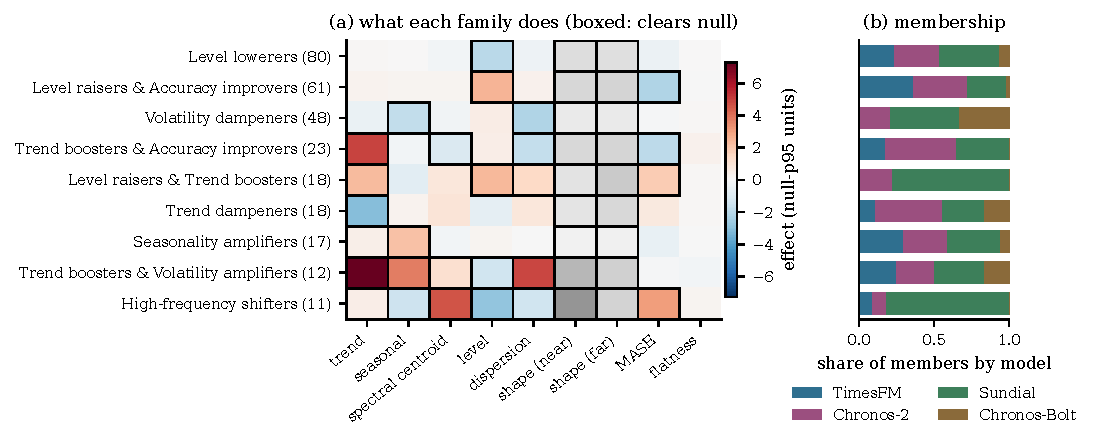
\includegraphics[width=\textwidth]{figures/families.pdf}
\caption{The nine causal-effect families of the example run, ordered by size. (a) Family centroid in
null units: what removing a member does, negated to state what the feature \emph{does}; red raises the
channel and blue lowers it. Boxed cells clear the null in the family description. The near- and
far-horizon shape channels are distances, drawn unsigned in gray. (b) Membership by model: families are
populated unevenly by model. Source: \texttt{sae/concept\_families.json}; regenerated by
\texttt{paper/figures/make\_figures.py}.}
\label{fig:families}
\end{figure}

\paragraph{The concepts are graded, not discrete.} Three observations indicate that ``concept'' should be
read as a region of a continuous effect space rather than as a discrete unit. First, clustering within a
layer rarely finds modules: 24 of 29 targets are non-modular, yielding only 9 per-target concepts. Second,
the strict atlas assigns only 86 of 293 features (29\%) to its 27 concepts. Third, the nine readable
families cover 288 of 293 features (98\%) but do \emph{not} beat a column-shuffle null (permutation
$p=1.0$ for the number of families and $p=0.985$ for coverage). A similar picture holds on the reference run,
where silhouette is 0.31--0.35 for every family count from 3 to 16 (\fid{CA-10}), and the 9-channel
ablation fingerprints have a participation-ratio dimension of only 2.09 (\fid{MN-07}). The families are
therefore a useful vocabulary for reading the report, and the paper uses them in that sense only.

\paragraph{Concepts named after ground truth are rare, and naming them requires a null.} Because the
benchmark records every generative component, \tool{} can ask whether a feature tracks a known field.
Some do: after dead-feature revival, 154 of 10{,}240 TimesFM features and 115 of 6{,}144 Chronos-T5-Base
features match a ground-truth field beyond a permutation null, the best being a Chronos feature tracking
intermittency at $\rho=0.881$ (\fid{MP-06}). But raw correlations do not separate trained from untrained
weights (an untrained twin scores 0.565 against 0.567), so only the margin over the null is evidence. Two
tempting stronger claims failed their tests. Validating concepts by moving a generator knob and watching the
concept respond was a confirmed negative, twice: 0 of 98 and then 0 of 151 knob--concept pairs survived
correction, because a knob moves any active feature about as much as the targeted one (\fid{MN-17}).
And a vivid TimesFM ``random walk'' concept (19 of 20 top series from the random-walk archetype; ablation
worsens MASE by 4.04 times the null) failed the seed-stability test and is not promoted (\fid{PM-11}).

\paragraph{Answer to RQ1.} TSFMs contain sparse, causally effective directions, and what they control is
mainly the level, volatility and shape of the forecast, with trend and seasonality handled by smaller
groups. These directions form a continuum with a few dominant axes rather than a set of discrete, named
concepts, and they are not specific to the generative factors a practitioner would name.

\subsection{RQ2: Are concepts shared across architectures?}
\label{sec:rq2}

\paragraph{Geometry is shared above chance, but ``similarity'' has no single meaning.} Peak linear CKA
between TimesFM and each other model is 0.38--0.43, against a shuffled-series null of 0.037, and the
TimesFM/Chronos-2 peak replicates on private data (dev 0.4262; private 0.4253 [0.4162, 0.4423]). The same
above-null band holds across five unrelated architectures, including Timer through the zero-code adapter
(0.449, null 0.063) and Lag-Llama (\fid{SH-01}). The three models with 16-step tokens are far more similar to
each other (0.909--0.928). Figure~\ref{fig:similarity} shows, however, that seven pair-similarity metrics
rank the six pairs inconsistently (Kendall's $W=0.28$, permutation $p=0.07$). TimesFM/Chronos-2 is the most
similar pair by error agreement (Spearman 0.947 across series), and only fourth by CKA and stitching gain.
\tool{} therefore never pools the metrics into one similarity score. Two further controls limit what
similarity means. An untrained pair of the same architecture is more CKA-similar (0.878) than a genuinely
related trained pair (0.734; difference $p=0.0005$), so representational similarity cannot detect model
lineage (\fid{MN-01}). And an attractive unit-level correspondence measure rose, rather than fell, when both
bases were randomly rotated (0.148 to 0.331), because TSFM layers are so low-rank (participation ratio as
low as 1.54) that every direction correlates with the same few components (\fid{SH-19}).

\begin{figure}[t]
\centering
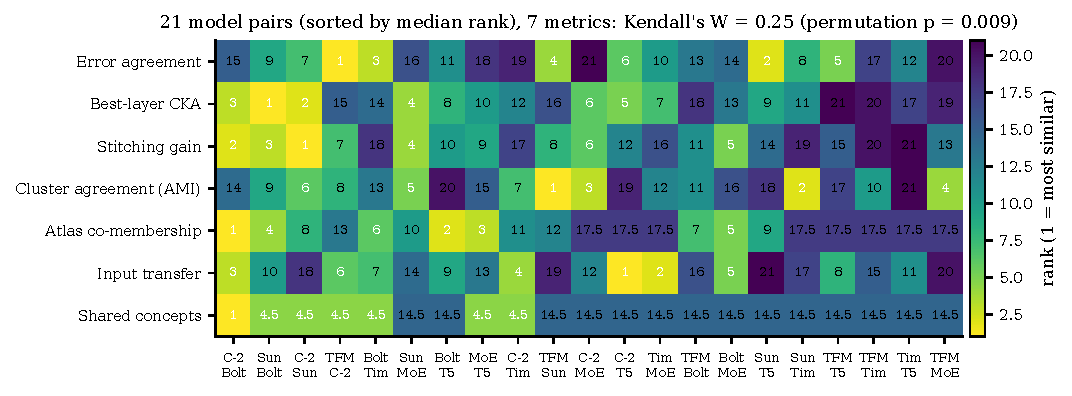
\includegraphics[width=0.66\textwidth]{figures/similarity.pdf}
\caption{Rank of each model pair (columns) under seven similarity metrics (rows); 1 is most similar.
Behavioral, geometric, translational, clustering and concept-level metrics disagree about which models are
alike. Source: \texttt{report/model\_similarity.json}.}
\label{fig:similarity}
\end{figure}

\paragraph{Models agree on which inputs a concept groups.} Concept transfer asks whether another model has a
feature that picks out a concept's top series. At atlas scale, 1{,}223 of 1{,}581 transfer tests (77\%) are
reciprocal after Benjamini--Hochberg correction. Twenty claims were registered from dev results alone and
tested once on the 800 private series: all 20 were confirmed under Holm correction (maximum adjusted
$p=0.0100$; private AUC 0.971--0.995 against null 95th percentiles of 0.57--0.77; Figure~\ref{fig:heldout}b).
This result has now replicated on three independent private draws: 19 of 20 in search mode on v1 epoch~1,
20 of 20 with frozen feature pairs on epoch~2, and 20 of 20 on v2 (\fid{SH-18}). Two caveats bound it. It is
an \emph{input-level} claim (the same series are grouped by both models), not a causal one. And the 20 v2
claims come from only two concepts, with only 6 of 20 private best features identical to the dev ones, so
the replicated statement is that the destination layer has \emph{some} feature that selects the same
series.

\paragraph{Models rarely agree on what a concept does.} Figure~\ref{fig:funnel} follows the candidates up
the evidence ladder. Of the 27 atlas concepts, 16 contain causal members from at least two models, but only
two are \emph{shared} (same effect and same inputs) and one is partially shared. The dominant class is
\emph{convergent} (13 concepts): features in different models have the same causal effect on
\emph{different} series. Eleven concepts belong to a single model. Restricted to the 22 seed-stable
concepts, the counts are 9 convergent, 10 single-model, 2 shared and 1 partially shared. No concept has
causal members in all four models; one spans three. The direct test agrees. Of the 1{,}223 reciprocal
transfers, 420 are scorable (both sides clear their own null on the shared series), and among those only 11
(2.6\%) show the same causal effect, 81 agree on level or shape alone, 264 show no specific agreement, and
64 (15.2\%) act measurably differently. The family memberships in Figure~\ref{fig:families}b tell the same
story: the families are segregated by model.

\begin{figure}[t]
\centering
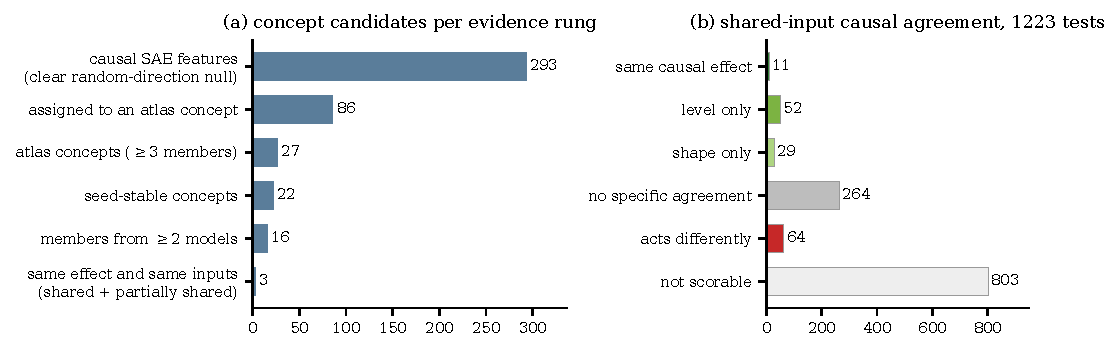
\includegraphics[width=\textwidth]{figures/funnel.pdf}
\caption{(a) Number of concept candidates at each rung. The first three bars count features and concepts
in sequence; the last three are separate properties of the 27 atlas concepts. (b) Verdicts of the
shared-input causal agreement test over all 1{,}223 reciprocal-FDR transfers; ``acts differently''
requires a lower-tail result against matched floors. Source: \texttt{sae/concept\_stage.json}.}
\label{fig:funnel}
\end{figure}

\paragraph{Answer to RQ2.} Different TSFMs \emph{detect} the same things: a concept learned by one model
selects series that another model's dictionary also selects, reliably enough to replicate on sealed data.
They mostly do not \emph{use} them the same way: effects shared on the same inputs are rare, the typical
multi-model concept is convergent, and no concept is common to all four models. Whole-layer similarity
metrics cannot reveal this distinction, and they disagree with each other.

\subsection{RQ3: Do concepts causally affect the forecast, and how much?}
\label{sec:rq3}

The ablation battery establishes causality at the level of single features: every concept in
Section~\ref{sec:rq1} is built from features that move the forecast more than a matched random removal does,
on the series they fire on, with reach verified. How much of the forecast these features account for is
a separate question, and the answer is: individually, little. On the reference run, the median effect of
removing one feature is 0.0395 context standard deviations, while replacing the layer by its SAE
reconstruction already moves the forecast by 0.139, 3.5 times more (\fid{MN-15}). Of 565 features that the
report would otherwise display as ``interesting'' because they activate strongly, 364 (64.4\%) clear no
causal channel at all (\fid{MN-14}); \tool{} collapses them rather than rendering them as findings. Causality
also depends on the dictionary: reviving dead atoms, which improves fidelity, reduced ground-truth
alignment at every TimesFM depth tested (from $-0.030$ to $-0.132$) while the causal signal fell much less,
and rose in one Chronos-2 layer (2.27 to 4.06 times chance; \fid{MN-21}).

Head-level analyses show the same gap between what looks important and what is. The correlation between
the attention mass a head places on seasonal lags and the seasonal power lost when that head is ablated is
$\rho=0.026$ in TimesFM and $\rho=-0.118$ in Chronos-T5-Base (\fid{CA-04}), in line with the
language-model finding that attention weights are not explanations \citep{jain2019attention}. A minimal
circuit restoring seasonality under \texttt{deseasonalize} consists of one head in TimesFM ($p=0.04$) but
five non-additive heads in Chronos-T5-Base ($p=0.008$; \fid{CA-03}).

\paragraph{Answer to RQ3.} Yes, causally, in the controlled sense: individual features and heads change the
forecast in specific, null-beating ways. But no single feature carries much of the forecast, most
prominent features carry nothing, and attention patterns are unreliable guides to which components matter.
Causal claims about TSFM concepts are claims about small, distributed contributions.

\subsection{RQ4: Where in depth, and how comparable is depth?}
\label{sec:rq4}

The corruption fingerprints locate where each model's activations react to a structural change of the
input, and their cross-model agreement is one of the most robust results in the ledger. For the registered
pair TimesFM/Chronos-2, all nine per-corruption agreements replicate on private data (overall $\rho=0.510$
[0.489, 0.527]; Figure~\ref{fig:heldout}a): the two models react at \emph{matching} depths to detrending,
deseasonalizing, frequency shifts and dropout, and at \emph{opposite} depths to noise ($\rho=-0.742$),
spikes ($-0.780$), warps ($-0.658$) and smoothing ($-0.466$). Whole-layer restoration can hide depth
structure: in TimesFM it is flat across depth, yet per window it concentrates in the window just before the
horizon and intensifies with depth (for \texttt{noise}, from 0.068 at layer 0 to 0.412 at layer 16;
\fid{DE-01}).

Comparing depth \emph{locations} across architectures, however, needs two qualifications that \tool{}
computes and renders for every run. The captured share of a forecast's computation ranges from 22\%
(Sundial, whose sampled head runs outside the captured pass) to 98\% (Chronos-2), and for Chronos-T5-Base,
where 100\% of encoder blocks are captured, it is only 14\% (\fid{DE-05}). And on a whole-stack depth axis,
Chronos-T5's last encoder block sits at 0.478, so the comparable depth range with TimesFM is only half the
axis (\fid{DE-04}). Which layers are ``interesting'' also depends on the selector: a specification curve over
three selectors found no selected layer robust for any model (\fid{DE-08}). Across a five-size Chronos-T5
scaling ladder (8M to 709M parameters), only family decodability increased monotonically with size
(\fid{DE-07}).

\paragraph{Answer to RQ4.} Depth-resolved reaction profiles are reproducible and reveal which structural
properties two models process at the same relative depth. Absolute depth locations are comparable across
architectures only after accounting for captured compute and for the depth convention, which \tool{} reports
alongside every depth claim.

\subsection{What replicated on held-out data}
\label{sec:heldout}

\begin{figure}[t]
\centering
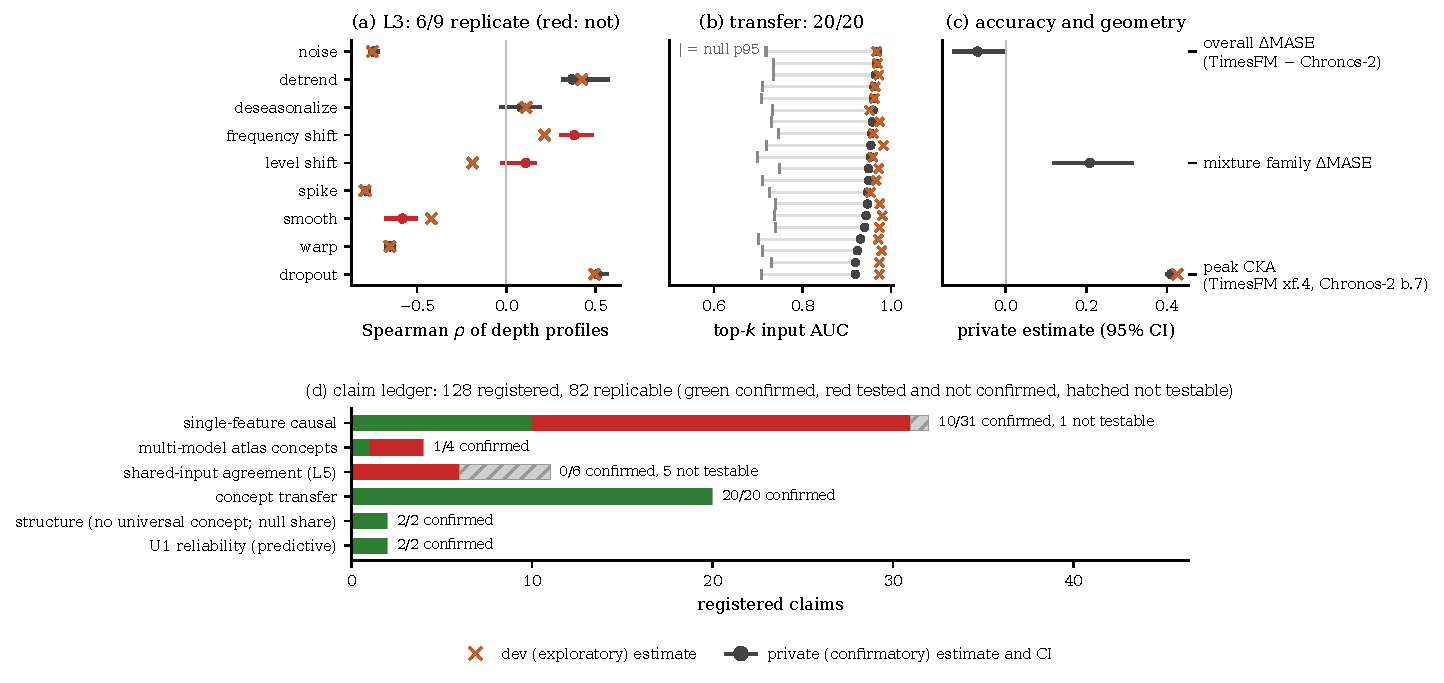
\includegraphics[width=\textwidth]{figures/heldout.pdf}
\caption{Every claim re-tested on the 800 sealed private series. (a) Per-corruption depth-profile agreement
between TimesFM and Chronos-2; (b) the 20 registered concept-transfer claims, with each claim's private null
95th percentile; (c) accuracy and peak CKA. Crosses: dev estimates; dots and bars: private estimates with
95\% series-bootstrap intervals. Source: \texttt{confirm/confirmation.json}.}
\label{fig:heldout}
\end{figure}

The \texttt{register} stage recorded 47 hypotheses, 31 of which the \texttt{confirm} stage can currently
re-test (L2 stitching, archetype-level accuracy and clustering claims are registered but not yet
replicable, and the report lists them as such). Every re-tested claim held (Figure~\ref{fig:heldout}): the
registered accuracy claim (Chronos-2 more accurate on \texttt{mixture}, $\Delta$MASE 0.307 [0.209, 0.413],
$p_{\text{Holm}}=0.0005$, $n=240$, where the minimum detectable effect had been 0.155), the peak-CKA pair, all
nine perturbation agreements and all 20 concept-transfer claims. Table~\ref{tab:results} collects the headline
results with their evidence class and status. What did \emph{not} undergo held-out testing matters equally:
the causal concept results of Sections~\ref{sec:rq1}--\ref{sec:rq3}, including the sharing classes and the
shared-input agreement counts, are exploratory. They were, however, reproduced on a second corpus: on the
v1 reference run, 0 of 19 atlas concepts span all four models, convergent is again the most common class,
and 12 of 89 scorable shared-input tests act differently (\fid{SH-16}, \fid{CA-06}).

\begin{table}[t]
\centering
\footnotesize
\setlength{\tabcolsep}{3pt}
\begin{tabularx}{\textwidth}{@{}l>{\raggedright}Xllll@{}}
\toprule
RQ & Result (example run unless an ID is given) & Evidence class & Status & ID \\
\midrule
1 & 293 causal features; 9 families, largest act on level/volatility & causal within-model & exploratory, 2 corpora & CA-10 \\
1 & Families cover 98\% but do not beat a shuffle null ($p=1.0$) & descriptive & exploratory, 2 corpora & CA-10 \\
1 & Knob-specific concept mediation: 0/98, then 0/151 & correlational & confirmed negative & MN-17 \\
2 & Peak CKA 0.425 vs null 0.037 & geometric & held-out confirmed & SH-01 \\
2 & 7 similarity metrics disagree ($W=0.28$) & mixed & exploratory & SH-05/06 \\
2 & Untrained pair more similar than related trained pair & geometric & confirmed negative & MN-01 \\
2 & Concept transfer on inputs: 20/20 & correlational & held-out confirmed (3 draws) & SH-18 \\
2 & No 4-model concept; convergent is the modal class & causal, compared & exploratory, 2 corpora & SH-16 \\
2 & Same effect on same inputs: 11/420 scorable & causal on shared inputs & exploratory, 2 corpora & CA-06 \\
3 & Feature effect 3.5$\times$ below SAE reconstruction cost & causal within-model & exploratory & MN-15 \\
3 & 64\% of prominent features causally null & causal within-model & exploratory & MN-14 \\
3 & Attention mass uncorrelated with head causality & causal vs.\ descriptive & exploratory & CA-04 \\
4 & Depth-profile agreement, 9/9 corruptions & causal within-model & held-out confirmed & CA-01 \\
4 & Captured compute 14\%--98\% qualifies depth claims & descriptive & confirmed & DE-05 \\
\midrule
L0 & Chronos-2 more accurate than TimesFM ($-0.148$) & behavioral & held-out confirmed & PM-05 \\
\bottomrule
\end{tabularx}
\caption{Headline results with evidence class and confirmation status. Each ID links to its entry in
\repo{FINDINGS.md}, which gives exact numbers, the reproduction command and the artifact path.}
\label{tab:results}
\end{table}

\FloatBarrier
\section{Using and Extending \tool{}}
\label{sec:usage}

A typical session installs the two packages, builds a benchmark and runs one configuration:
\begin{center}
\begin{minipage}{0.95\textwidth}
\footnotesize
\begin{verbatim}
pip install -e . && pip install -e tsfm_lens
cd tsfm_benchmark && PYTHONPATH=. python3 example_runs/run_full.py \
       --config configs/example.yaml --out ./benchmark_out --references monash
cd ../tsfm_lens && python run.py --config configs/examples/medium_2model.yaml
\end{verbatim}
\end{minipage}
\end{center}
The CLI adds a preflight check (\texttt{-{}-doctor}), partial reruns (\texttt{-{}-stages}, \texttt{-{}-force}),
checks for new checkpoints or library upgrades (\texttt{-{}-check-alignment}, \texttt{-{}-check-adapter}) and an
environment diff (\texttt{-{}-verify-provenance}). A CPU-only mock configuration runs every stage in minutes in continuous
integration, and the worked example (\repo{tsfm_lens/docs/worked_example.md}) walks through a report. The seven-model analysis records
21.1 GPU-hours of stage time, mostly SAE training and the concept battery; stages through L3 take about 1.4 hours. Of eight
TSFM checkpoints probed, two (Timer, Time-MoE) load through the zero-code path and five with standalone packages
need a hand-written adapter (\fid{MN-25}), for which a template, a conformance check
(\texttt{-{}-check-adapter}) and a guide with a pitfall checklist (\repo{tsfm_lens/docs/ADDING_A_MODEL.md}) exist. New report sections declare their artifact requirements, new claims must use the
typed \texttt{Finding} record, and new configuration fields declare which artifacts they affect.

\section{Limitations}
\label{sec:limitations}

\paragraph{Models.} Seven transformer models with contiguous tokens; disjoint-lag tokens (Lag-Llama) get
reduced scope. Timer's features do not exceed chance, and with seven models, contrasts are confounded with architecture, size and
training data. The analysis is univariate: Chronos-2's cross-series group attention is not measured
(\fid{PM-13}), and Chronos-T5's decoder and Sundial's flow head are not captured.

\paragraph{Ground truth, external validity and confirmation.} Ground truth is exact only for the synthetic tier and
encodes our generators' assumptions; 12 of 33 concept parts are dominated by one real-derived generator, and pretraining
overlap cannot be verified. Real data are part of the analysis, not absent from it: 410 of the 965 dev series are real-derived
(Monash weather, ETT, and Chronos electricity and traffic) and the dictionaries are trained with 4{,}000 additional real
Monash windows. Raw real benchmarks are nonetheless a weaker bed for the causal questions: real rows give TimesFM
representations of lower effective dimension than the synthetic corpus (1.76 against 2.66) and more dead dictionary
atoms (\fid{MN-20}); weakly predictable real-derived series receive flat forecasts in 67--100\% of cases, where an
ablation has nothing to move (\fid{BM-06}); real series carry no generative ground truth; and public archives may be in
the models' pretraining data. A full run on a large raw benchmark such as GIFT-Eval remains to be done; the pipeline runs
on any sealed corpus. Held-out confirmation covers accuracy, geometry,
perturbation agreement, transfer, single-feature causal effects, atlas structure and failure prediction, on one private
split opened once (a second look needs a fresh epoch), and the 20 confirmed transfers come from two source concepts.

\paragraph{Effect sharing on the same series.} The cross-model causal claims are the ones that did not confirm, and the
known-answer test explains why: the shared-input rung is specific but detects a planted shared concept across
architectures in at most 0.4 of seeds, and more shared series do not help (\fid{MN-30}). We therefore built the redesign
this diagnosis suggested (ablating a concept's member subspace on each side, an equal-rank size-matched null, and
interval estimates against matched floors) and fixed its pass criterion in advance: sensitivity $\ge0.8$ on both planted
shared concepts, false agreement $\le0.05$, on held-out seeds. It also fails (sensitivity 0.5 and 0.375, with 0 of 14
false agreements), and the reason is a ceiling rather than a design detail: even the planted distributed subspace itself
does not move the forecast more than an equal-sized random removal (\fid{MN-32}). Per-series agreement of causal
effects across architectures is therefore not measurable by ablation at the effect sizes these models have, and
\tool{} compares effects across models at the level of concept profiles instead (Section~\ref{sec:rq2}).

\paragraph{SAE dependence, usability and completeness.} Concept results depend on dictionary size, sparsity,
revival and seed; the system measures this dependence but cannot remove it, and feature death tracks layer
geometry (alive atoms scale with effective dimension with log-log exponent 1.02, $\rho=0.58$ over 45 cells;
\fid{MP-05}). Readability for newcomers is a design intention; no user study measured comprehension. Controls catch only failures
for which a known-answer case exists.

\section{Conclusion}
\label{sec:conclusion}

TSFM interpretability is harder than it looks: tokens mean different things in different models, there is no
annotated ground truth, and causal effects are small enough that measurement artifacts dominate unless controlled.
\tool{} addresses this with a controlled benchmark, measured alignment, null- and reach-gated causal concepts and a
register-then-confirm protocol, behind one command and a report designed to be understandable by newcomers. On seven
TSFMs, causal features form a compact vocabulary centered on forecast level and seasonality; different architectures
select the same inputs for a concept, replicably across four sealed draws, while organizing their causal machinery by
model; causal importance sits in a minority of features that activation prominence does not reveal; and depth
signatures replicate held-out. Each of these conclusions is stated with its evidence class, and each held-out claim
was registered before the private data were opened.

\paragraph{Availability.} Code (MIT), configurations, the example run and the findings ledger are at
\url{\repourl}; the \texttt{dev} branch holds the full research log and study drivers.


\acks{Computational resources were provided by the second author's lab at Rutgers University. This work received no external funding, and the
authors declare no competing interests. Use of AI tools: Claude (Anthropic) wrote most of the repository's code and tests, ran the experiments and helped draft and edit the manuscript, under the authors' direction. The research questions, ideas and general design choices are the authors', who reviewed the implementation details Claude proposed, checked every reported result and take full responsibility for the content.}

\appendix
\section{Findings Ledger Index}
\label{app:ledger}

The paper cites findings by identifier. Each identifier is an entry in \repo{FINDINGS.md}, which records
for every result its exact numbers, the models involved, its evidence class, its status (exploratory,
confirmed, held-out confirmed, negative), a reproduction pointer (configuration, command and artifact
path) and an interestingness score from 1 to 5. The ledger is curated from the research log on the
\texttt{dev} branch and includes negative results on equal terms. Section letters: SH shared vs.\ unique
representations; CA causal agreement; DE depth; PM per-model character; MP method positives; MN method
negatives; BM benchmark trust. Table~\ref{tab:ledger} indexes the entries cited here.

\begin{center}
\scriptsize
\setlength{\tabcolsep}{3pt}
\begin{longtable}{@{}l>{\raggedright}p{8.6cm}>{\raggedright}p{2.6cm}c@{}}
\caption{Ledger entries cited in this paper (score = interestingness, 1--5).}\label{tab:ledger}\\
\toprule
ID & Claim (abridged) & Evidence / status & Score \\
\midrule
\endfirsthead
\toprule
ID & Claim (abridged) & Evidence / status & Score \\
\midrule
\endhead
\bottomrule
\endfoot
SH-01 & Peak CKA 0.38--0.47 above shuffled-series nulls (0.02--0.16) across five architectures, including Timer via the zero-code adapter & geometric; exploratory & 5 \\
SH-05 & CKA and clustering AMI rank model pairs differently on three panels & geometric vs.\ descriptive; replicated & 5 \\
SH-10 & Joint crosscoder loses to independent post-hoc-matched SAEs (0.2787 vs.\ 0.3204, $p=0.002$), pre-registered & correlational; negative & 5 \\
SH-14 & Concept transfer on shared inputs vs.\ stratum-matched null: 56.3\% forward, 46.1\% reciprocal; uniform null gave false 30/30 & correlational; exploratory & 5 \\
SH-16 & No atlas concept spans all four models; convergent is the modal sharing class & descriptive over causal parts; exploratory & 5 \\
SH-18 & Registered concept-transfer claims confirmed on private data: 19/20, 20/20 frozen, 20/20 on v2 & held-out confirmed & 5 \\
SH-19 & Unit-level correspondence fails rotation controls (0.148 $\to$ 0.331); participation ratio as low as 1.54 & geometric; negative & 5 \\
SH-20 & 11 of 13 targets non-modular once a minimum cluster size is enforced & descriptive; confirmed & 4 \\
CA-01 & Perturbation-fingerprint agreement is pair-specific; TimesFM/Chronos-2 replicates on private data & causal within-model; held-out & 4 \\
CA-03 & Seasonality circuit: 1 head (TimesFM) vs.\ 5 non-additive heads (Chronos-T5-Base) & causal within-model; exploratory & 4 \\
CA-04 & Attention mass at seasonal lags uncorrelated with causal importance ($\rho=0.026$, $-0.118$) & causal vs.\ descriptive; exploratory & 4 \\
CA-06 & On shared inputs with matched floors, most apparent cross-model disagreement disappears (18/19 $\to$ 12/89) & causal on shared inputs; exploratory, 2 corpora & 5 \\
CA-07 & Median level share of a causal feature's effect 0.535; most features shape-causal beyond a level-removed null & causal within-model; exploratory & 4 \\
CA-10 & Causal effect space is a continuum; families tile it but do not beat a shuffle null & descriptive; exploratory, 2 corpora & 4 \\
DE-01 & Whole-layer patching hides a depth-intensifying recency effect in the last pre-horizon window & causal within-model; exploratory & 4 \\
DE-03 & Chronos-2 skip lens was a silent no-op (identical MASE at 12 layers); corrected reach 0.737 $\to$ 0.000 & causal within-model; confirmed & 5 \\
DE-04 & Chronos-T5 encoder ends at depth 0.478 on a whole-stack axis; 50\% comparable overlap with TimesFM & descriptive; confirmed & 5 \\
DE-05 & Captured share of forecast FLOPs: 14.35\% (Chronos-T5-Base) to 97.5\% (Chronos-2) & descriptive; confirmed & 5 \\
DE-07 & Chronos-T5 scaling ladder: only family decodability scales monotonically & mixed; exploratory & 5 \\
DE-08 & Layer selection depends almost entirely on the selector (0/3 robust layers) & descriptive; confirmed & 4 \\
PM-05 & Chronos-2 most accurate and best observed; winners vary by family; held-out on v2 & behavioral; partly held-out & 4 \\
PM-07 & Models differ ${\sim}5.4\times$ in reversion to the mean; flat forecasts driven by weakly predictable data & behavioral; confirmed on run & 4 \\
PM-08 & Random-weight twins are not one null: identity stack (TimesFM) vs.\ dead forecasts (Chronos-2/Bolt) & architecture fact; confirmed & 5 \\
PM-09 & Sundial scorable as causal destination 1/71 $\to$ 12/71 after seeding fix & causal; corrected & 3 \\
PM-11 & Causally load-bearing TimesFM random-walk concept fails seed stability & causal within-model; unstable & 3 \\
PM-13 & Chronos-2 group attention unmeasured by design & scope statement & 3 \\
PM-15 & Sundial adapter bypassed checkpoint normalization; residual 38.43 $\to$ 0.030 & behavioral; fixed & 4 \\
MP-01 & Token spans can be measured (IoU 1.0 on 6 checkpoints); zero-code adapter follows & method; confirmed & 5 \\
MP-02 & Alignment gates must be normalized by their attainable ceiling & method; confirmed & 3 \\
MP-03 & AuxK revival recovers dead SAE atoms 10--13$\times$ on real activations & method; adopted & 4 \\
MP-04 & Single-seed SAE gold ranking flips a bake-off verdict; 3 seeds fix it & method; fixed & 5 \\
MP-05 & SAE feature death set by layer geometry (exponent 1.02), not recipe & correlational; replicated & 5 \\
MP-06 & Ground-truth alignment of SAE features is real only over a permutation null & correlational; exploratory & 3 \\
MP-07 & Ablation battery discriminates: 2.49--6.61$\times$ chance & causal within-model; confirmed & 4 \\
MP-09 & Dev and private splits exchangeable (energy $p=0.51$; TOST 21/22) & held-out validation & 3 \\
MN-01 & Similarity cannot detect lineage: untrained pair 0.878 $>$ trained related pair 0.734 & geometric; negative & 5 \\
MN-05 & Residualizing on provenance made 93\% of headline cards float-rounding noise & method; fixed & 5 \\
MN-06 & A grounded small LLM narrator fabricates comparisons; guards do not converge & method; negative & 5 \\
MN-07 & Causal fingerprints are nearly one-dimensional (PR 2.09) & causal, compared; negative & 4 \\
MN-14 & 64.4\% of visually prominent SAE features are causally null & causal within-model & 4 \\
MN-15 & SAE reconstruction moves the forecast ${\sim}3.5\times$ more than removing a feature & causal within-model & 4 \\
MN-16 & ``Reconstruction beats clean forecast'' replicated in 1/5 seeds; retracted & causal; retracted & 4 \\
MN-17 & Generator-counterfactual concept mediation: 0/98 and 0/151 & correlational; negative & 5 \\
MN-18 & Absence of agreement is not disagreement: 109/288 $\to$ 9 & method; fixed & 4 \\
MN-19 & ``Same inputs'' must be top-$k$ overlap, not whole-series correlation & method; fixed & 4 \\
MN-21 & Reviving dead features hurts ground-truth alignment in TimesFM at every depth & correlational vs.\ causal; exploratory & 5 \\
MN-23 & MASE denominator floors out on intermittent series & metric caveat & 3 \\
MN-24 & A precision mismatch left aggregates intact but reorganized 71\% of a partition & method; fixed & 4 \\
MN-25 & Zero-code adapter resolves 2 of 8 probed TSFM checkpoints & descriptive; open & 3 \\
BM-05 & Counterfactual identity check caught a corruption-replay bug (244/298 $\to$ 0/1113) & benchmark; fixed & 2 \\
BM-06 & ${\sim}$42\% of the v1 dev corpus is weakly predictable real-derived data and drives the flat-forecast share & behavioral; measured & 4 \\
\end{longtable}
\end{center}

\section{Statistical Details}
\label{app:stats}

\paragraph{Paired series bootstrap.} For models $a,b$ and series $s=1,\dots,n$ with per-series scores
$m_{a,s}, m_{b,s}$, let $d_s=m_{a,s}-m_{b,s}$ and $\bar d=\frac1n\sum_s d_s$. For $B=n_{\text{boot}}$ resamples
$s^{*}\sim\mathrm{Unif}\{1..n\}^n$, $\bar d^{*}_b=\frac1n\sum_i d_{s^*_i}$. The interval is the percentile
interval of $\{\bar d^*_b\}$, and the two-sided $p$-value is
$p=\min\!\Big(1,\max\!\big(\tfrac1B,\;2\min\{\tfrac1B\#(\bar d^*_b\le 0),\,\tfrac1B\#(\bar d^*_b\ge 0)\}\big)\Big)$
(\texttt{analysis/stats.py::paired\_bootstrap}). The floor at $1/B$ follows \citet{phipson2010permutation}.

\paragraph{Cluster bootstrap for layer statistics.} Statistics computed from window-level activations (CKA,
fingerprints) resample series and keep all windows of a drawn series together, so dependence within a series
is preserved \citep{cameron2008cluster}.

\paragraph{Holm and BH.} For $m$ sorted $p$-values $p_{(1)}\le\dots\le p_{(m)}$, Holm's adjusted values are
$\tilde p_{(i)}=\max_{j\le i}\min\big(1,(m-j+1)p_{(j)}\big)$ \citep{holm1979}. With every $p\ge 1/B$, the
smallest attainable adjusted value is $m/B$; the multiplicity ledger reports it for every family and flags
families with $m/B>\alpha$. BH adjusted values are
$\tilde q_{(i)}=\min_{j\ge i}\min\big(1,\tfrac{m}{j}p_{(j)}\big)$ \citep{benjamini1995fdr}.

\paragraph{Row-matched ablation null.} For feature $i$ with row set $R_i$ and $J$ null directions
$u_j\sim\mathcal N(0,I)$, $u_j\leftarrow u_j/\|u_j\|$, the null forecast removes
$\bar a\,W_d u_j$ from the reconstruction, where $\bar a$ is the mean absolute activation removed by the
ablations in the same batch. Channel $c$ clears if
$\frac{1}{|R_i|}\sum_{r\in R_i}|\Delta^{(c)}_{i,r}| > q_{0.95}\{|\Delta^{(c)}_{u_j,r}|: j\le J,\,r\in R_i\}$.
A null with no spread (all draws exactly 0, which quantized decoding can produce) is reported as degenerate
and not scored.

\paragraph{Transfer AUC and its null.} For a source concept with top-$k$ series $S$ and a destination layer
with series-level feature activations $a_f$, the transfer statistic is $\max_f \mathrm{AUC}(a_f; S)$, the best
separation of $S$ from the other series by any destination feature. Its null draws random sets of $k$ series
matched on the strata of $S$ and recomputes the same maximum, so the search over features is included in the
null (a per-feature null would ignore the search and clear almost everything). The reverse leg takes the
chosen destination feature's own top-$k$ series and scores them by the source concept's activation, against
matched draws of that single statistic. Permutation $p$-values are $(1+\#\{\text{null}\ge\text{obs}\})/(1+n)$.
A registered claim combines the forward and reverse legs by $\max(p,p_{\text{rev}})$
(intersection--union) and is Holm-corrected across claims.

\paragraph{Shared-input agreement.} On the shared set $U$, both sides are ablated and scored with the
nine-channel battery, with level and shape separated. Statistic (i) is the Spearman concordance, across the
series of $U$, of the two sides' signed level effects; statistic (ii) is the cosine between the two sides'
level-removed shape vectors, each channel normalized by that side's own null $q_{0.95}$. For the floors, each
side draws random feature sets matched to its own activation on $U$, ablates them and re-scores the same
statistic against the other side's fixed, measured effect. A statistic agrees if it exceeds the $q_{0.95}$ of
both sides' floors; ``acts differently'' requires falling below the $q_{0.05}$ of both
(\texttt{sae/shared\_input\_agreement.py}).

\paragraph{Minimum detectable effect.} For a registered accuracy claim with private sample size $n$, the
confirm stage resamples per-series paired differences, recentred and shifted by a candidate effect,
applies the same paired bootstrap test to each simulated sample, and bisects for the smallest shift detected
with power 0.8 at $\alpha$ (capped at four standard deviations, reported as a boundary case), all
\emph{before} the private result is read (\texttt{analysis/power.py}).

\section{Reproducibility}
\label{app:repro}

\paragraph{Artifacts.} The example run \repodir{examples/concept_atlas_v2} contains the resolved configuration,
the rendered report, and the lightweight artifacts of every stage (JSON and parquet; activations and SAE
weights are omitted for size). \texttt{paper/figures/make\_figures.py} regenerates Figures
\ref{fig:heldout}, \ref{fig:families}, \ref{fig:funnel} and \ref{fig:similarity} from those artifacts, and
accepts \texttt{-{}-run} to point at any other run directory.

\paragraph{Commands.} From \texttt{tsfm\_lens/}:
\begin{center}
\begin{minipage}{0.95\textwidth}
\footnotesize
\begin{verbatim}
python run.py --config configs/concept_atlas_v2.yaml            # full run
python run.py --config configs/concept_atlas_v2.yaml --stages report
python run.py --verify-provenance runs/concept_atlas_v2         # env diff
python -m pytest tests -q                                       # test suite
\end{verbatim}
\end{minipage}
\end{center}
Building the v2 benchmark uses \repo{tsfm_benchmark/configs/README.md}. The private split used here was
opened once (2026-09-28); replicating the confirmation requires minting a fresh epoch.

\paragraph{Environment.} Python 3.12, numpy 2.1.0, PyTorch 2.9.1 (CUDA 13.0), transformers 4.57.6,
timesfm 2.0.2, chronos-forecasting 2.3.1, zarr 2.18.7 (zarr~3 stores read back empty under the v2 API) and
scikit-learn 1.9.0; the full pin list and the reason for each load-bearing pin is \repo{DEPENDENCIES.md}.
Each run records its environment in \texttt{run\_manifest.json}. The main-branch test suite passes (2{,}112
passed, 27 skipped for \texttt{tsfm\_lens}; 124 passed, 1 skipped for \texttt{tsfm\_benchmark}).

\paragraph{Runtime.} Table~\ref{tab:runtime} gives the wall-clock time per stage for the example run on one
NVIDIA RTX A5000 (24~GB) with four CPU threads.

\begin{table}[h]
\centering
\scriptsize
\setlength{\tabcolsep}{4pt}
\begin{tabular}{@{}lrlrlr@{}}
\toprule
Stage & seconds & Stage & seconds & Stage & seconds \\
\midrule
corpus & 1.5 & internals & 230.5 & attention & 34.7 \\
extract & 57.5 & lens & 12.9 & cluster & 22.3 \\
budget & 5.3 & l1 & 30.2 & sae & 8{,}593.9 \\
frontend & 8.6 & l2 & 86.0 & concepts & 13{,}376.7 \\
layer\_screen & 95.4 & l3 & 195.0 & exemplars, register & 2.5 \\
l0 & 207.5 & confirm & 131.0 & report & 59.5 \\
\midrule
\multicolumn{5}{@{}l}{Total} & 23{,}151 (6.43 h) \\
\bottomrule
\end{tabular}
\caption{Per-stage wall-clock time of the example run (\texttt{run\_manifest.json}). The concept stage
includes the shared-input agreement test (10{,}855 s) and three replicate SAE seeds per target (1{,}768 s).}
\label{tab:runtime}
\end{table}

\section{Report Walkthrough}
\label{app:report}

Figures \ref{fig:report-top}--\ref{fig:report-confirm} are unedited screenshots of the example report
(\repo{examples/concept_atlas_v2/report.html}), rendered with a headless browser.

\begin{figure}[p]
\centering
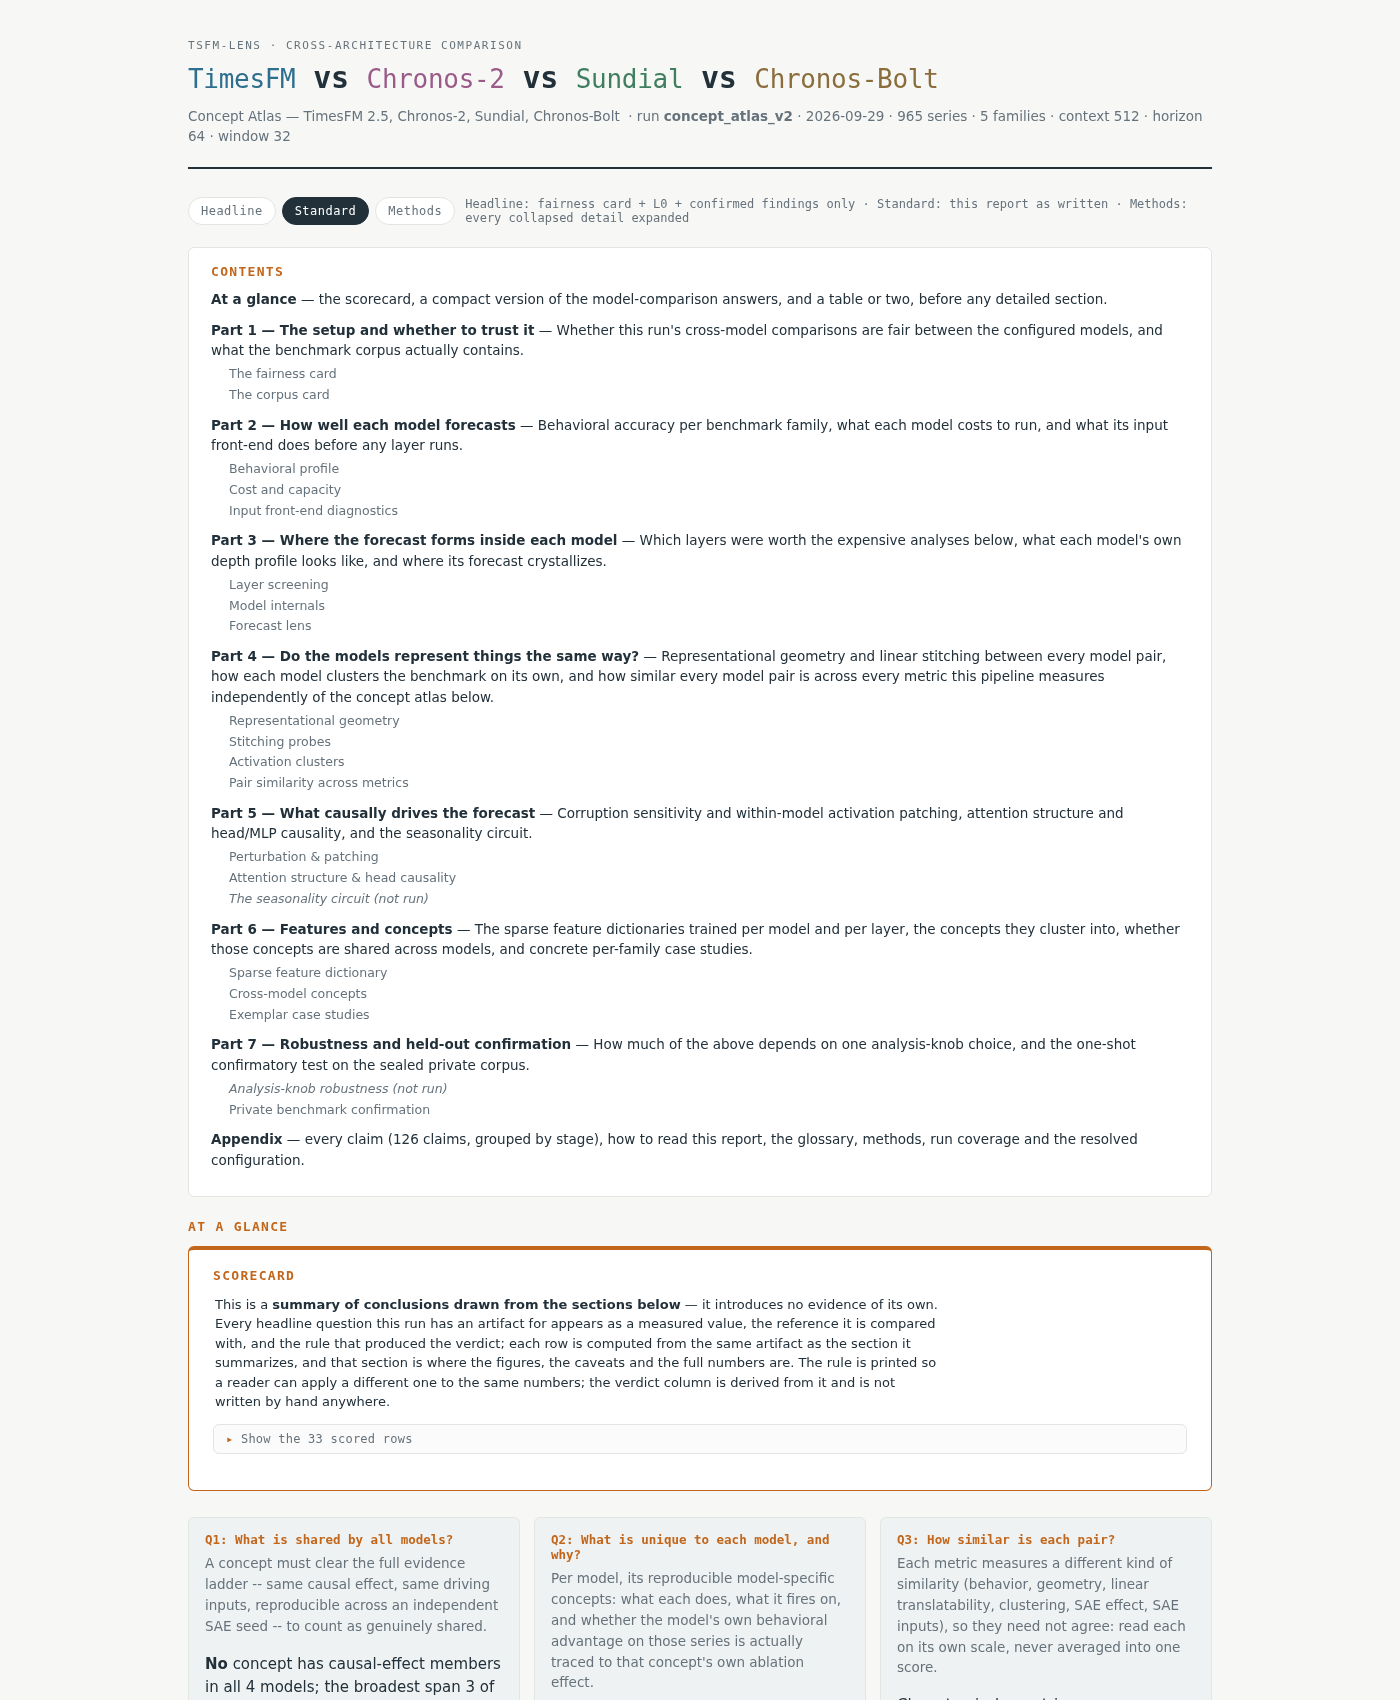
\includegraphics[width=0.86\textwidth]{figures/report_top.png}
\caption{Report opening: reading-level toggle (headline, standard, methods), the question-first table of
contents and the start of the derived scorecard and the three model-comparison answer boxes.}
\label{fig:report-top}
\end{figure}

\begin{figure}[p]
\centering
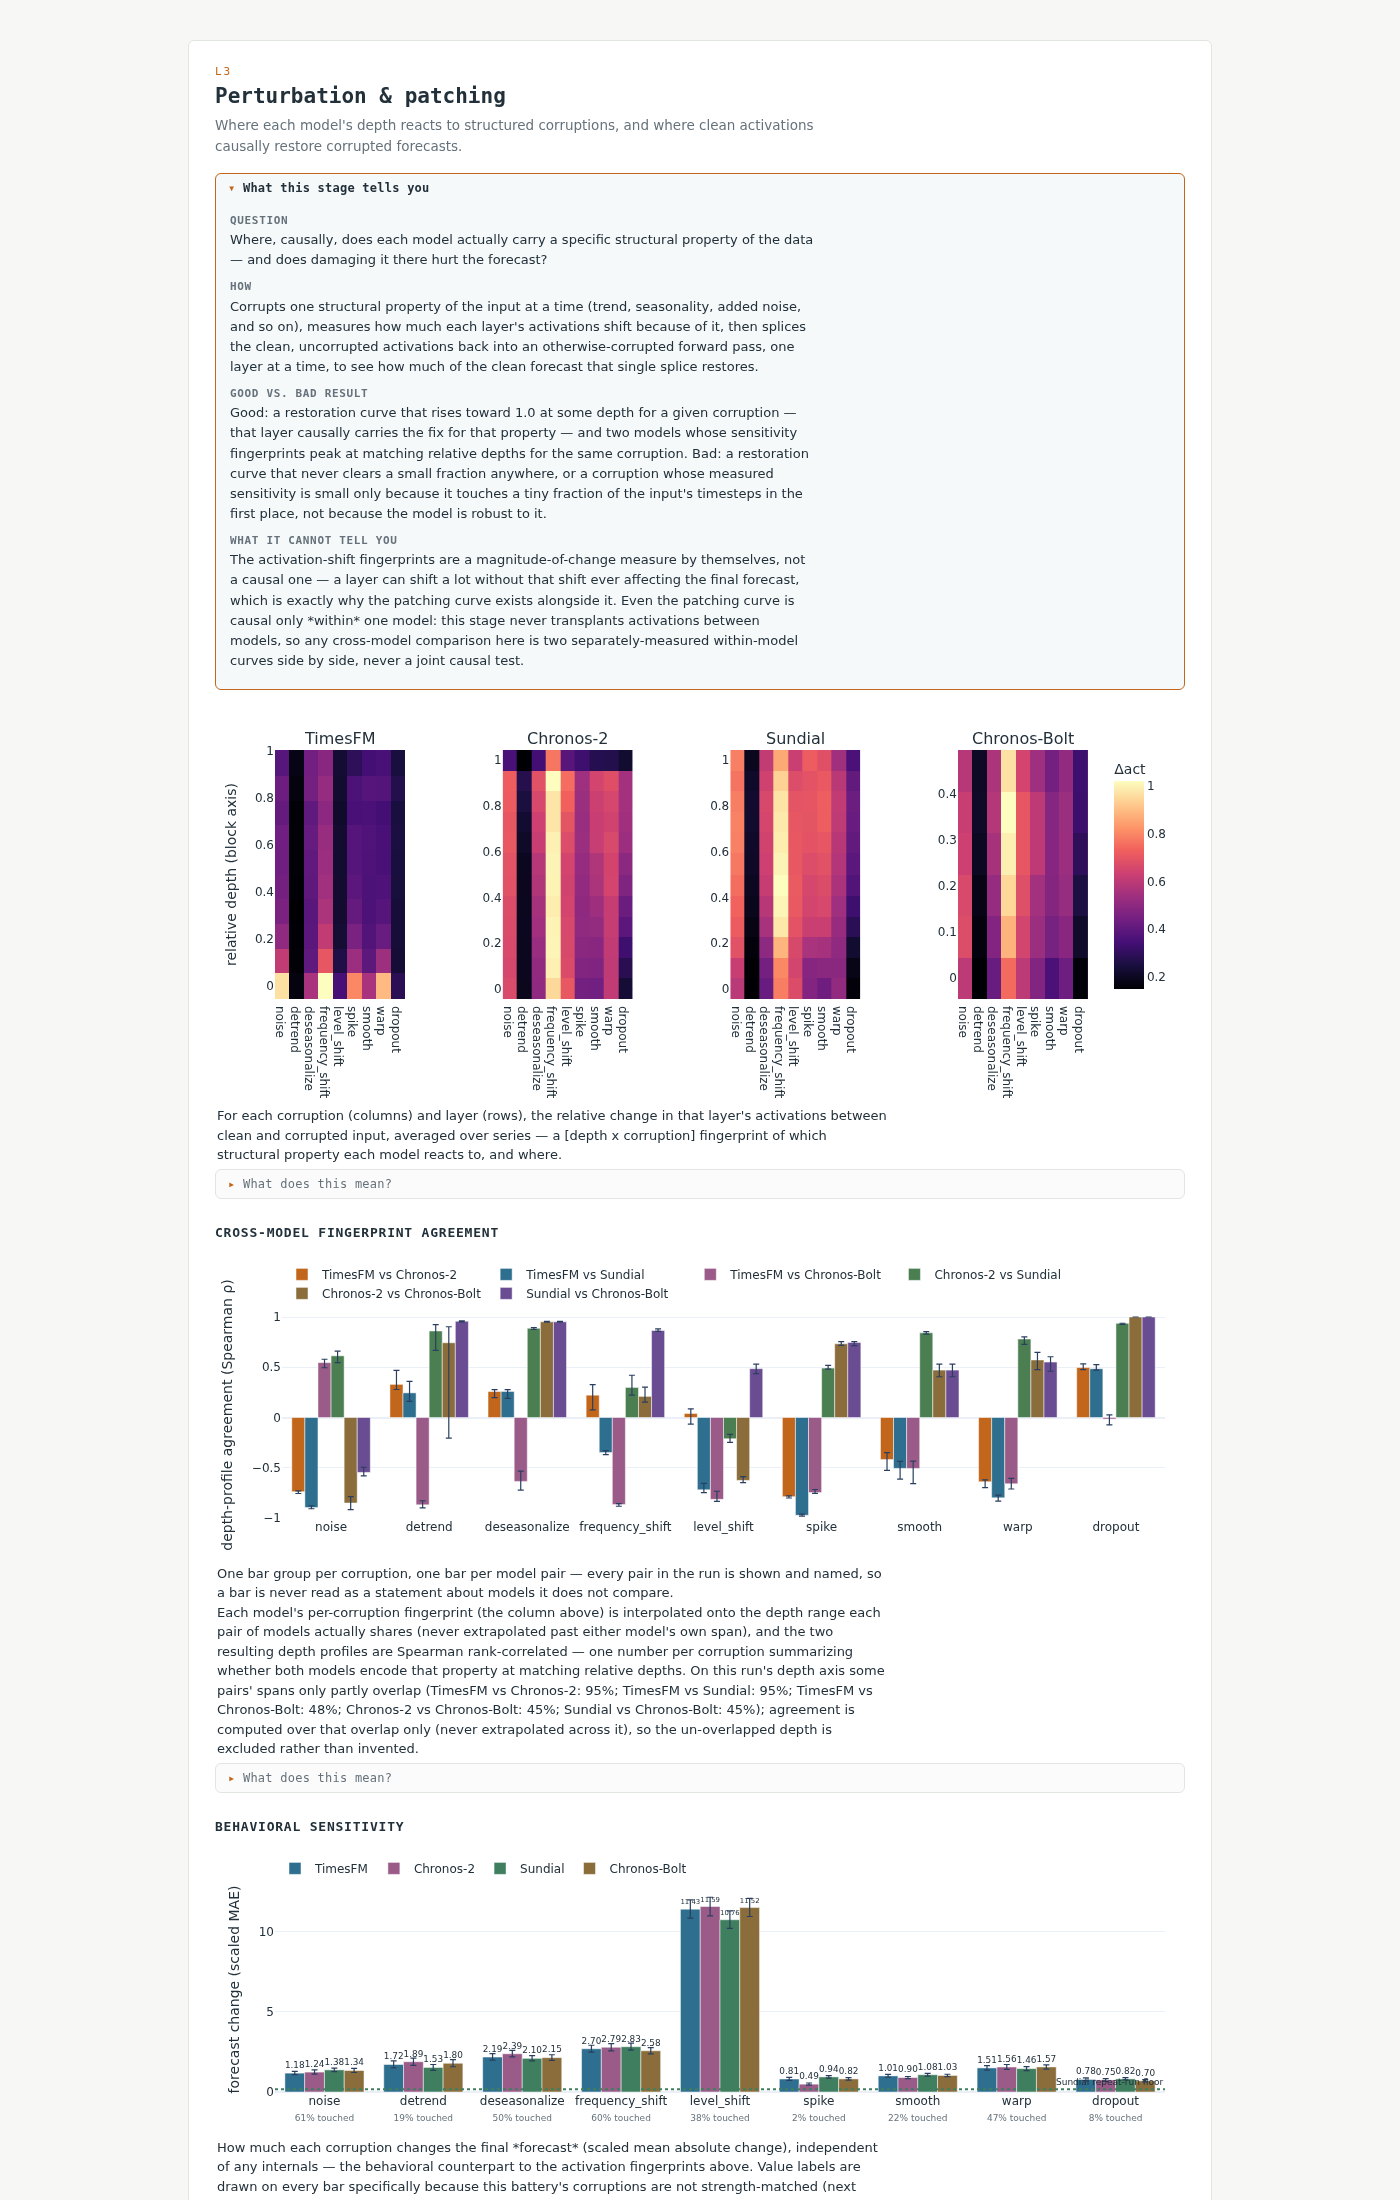
\includegraphics[width=0.86\textwidth]{figures/report_sec-l3.png}
\caption{A stage section (L3, perturbation and patching). The open card states the question, the method,
what a good and a bad result look like and what the analysis cannot tell you; each figure has a caption and a
collapsible ``What does this mean?'' note.}
\label{fig:report-l3}
\end{figure}

\begin{figure}[p]
\centering
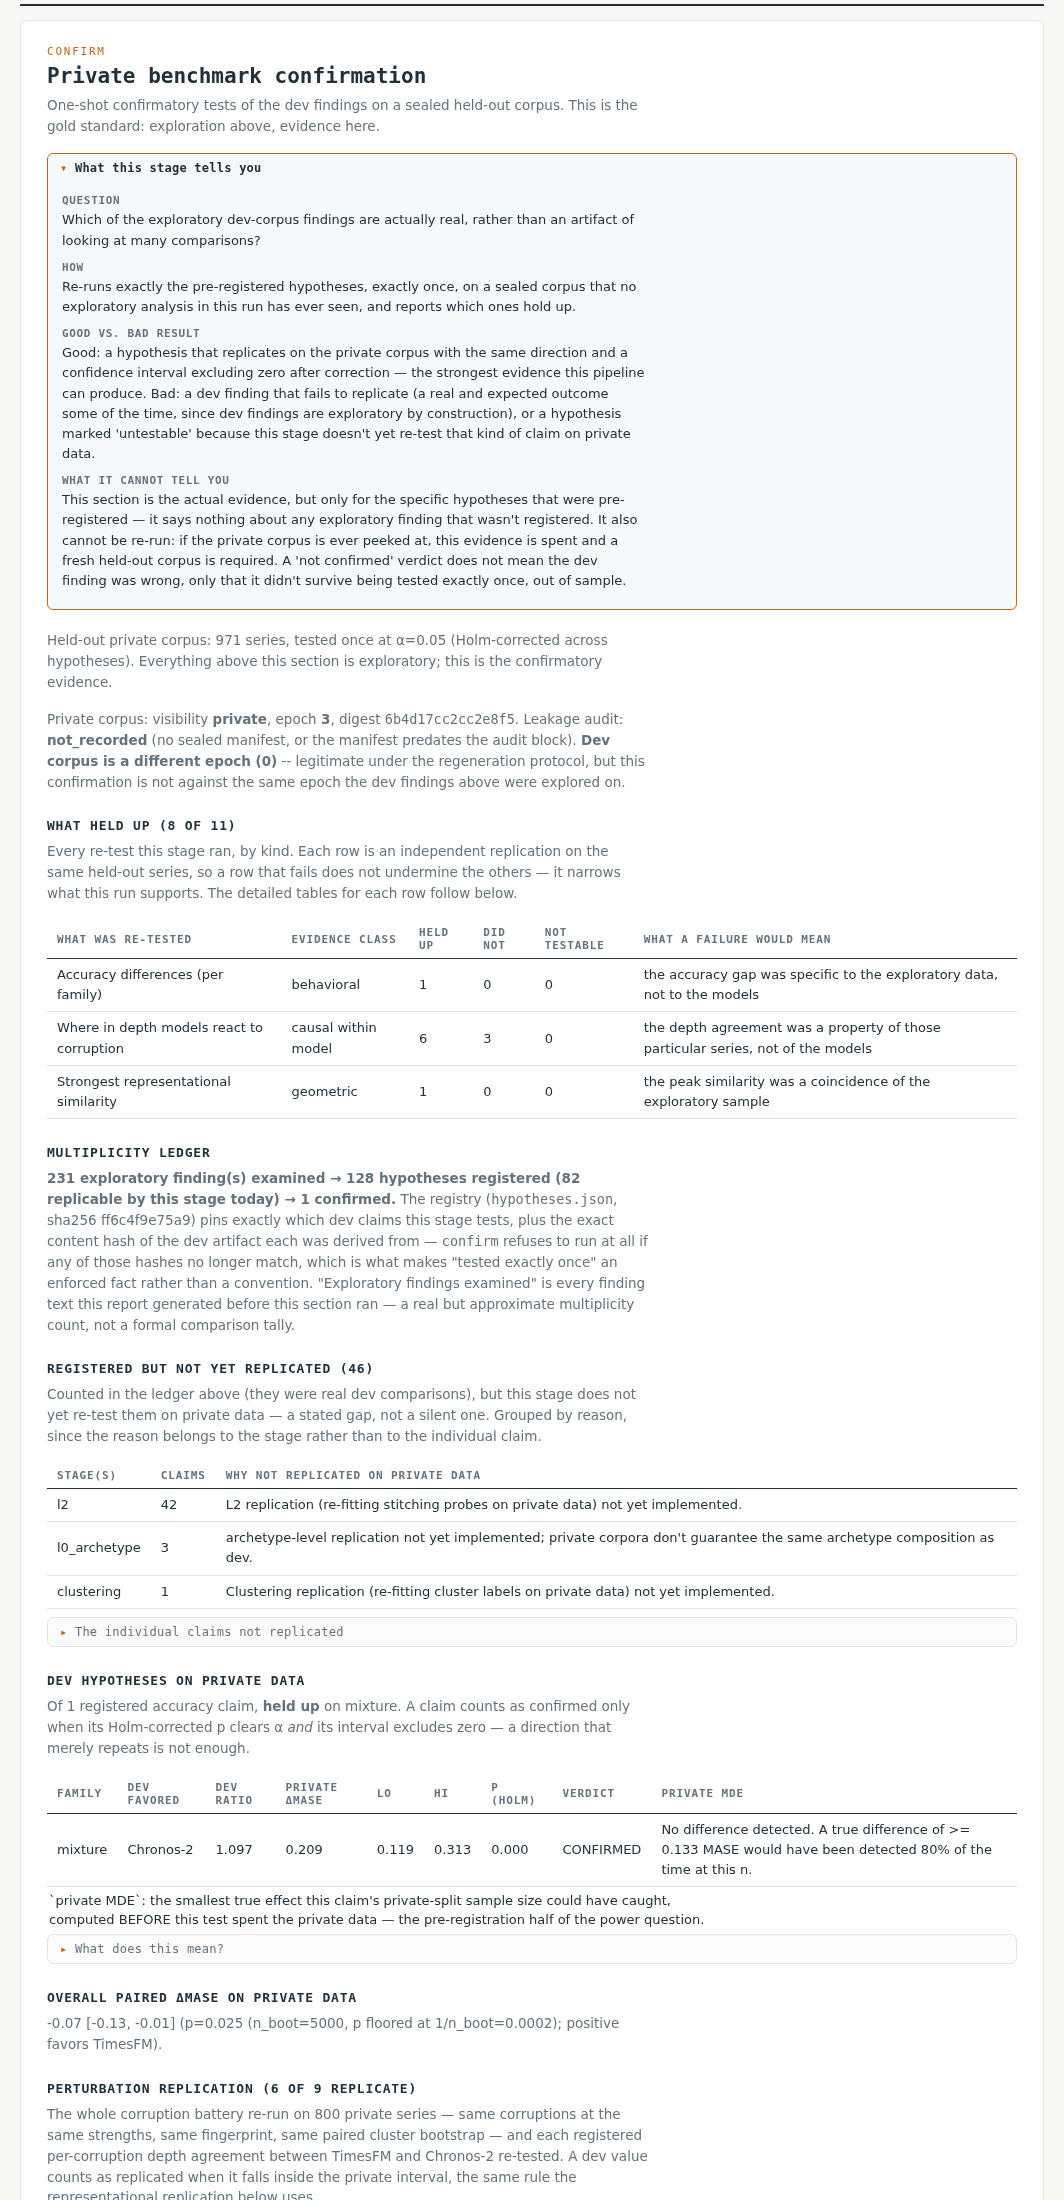
\includegraphics[width=0.86\textwidth]{figures/report_sec-confirm.png}
\caption{The confirmation section: what held up, the multiplicity ledger from exploratory findings to
registered and confirmed claims, registered claims not yet replicable with their reasons, and each
registered claim with its private estimate and pre-computed minimum detectable effect.}
\label{fig:report-confirm}
\end{figure}

\section{Adapter Pitfalls: a Worked Case}
\label{app:adapters}

The adapters guide (\repo{tsfm_lens/docs/ADDING_A_MODEL.md}) documents every pitfall we met. The most
instructive is the Sundial normalization bug (\fid{PM-15}), because the pipeline measured it correctly and
it was still misread.

\paragraph{What happened.} Many Hugging Face checkpoints normalize inputs only inside their own
\texttt{generate()} path. Sundial z-scores each series in \texttt{generate()}, but its \texttt{forward()}
defaults to no normalization. \texttt{generate()} was broken on the installed transformers version, so the
adapter called \texttt{forward()} directly and fed the model raw-scale input. The remote code's own
normalizing branch of \texttt{forward()} fails when more than one sample is drawn.

\paragraph{Symptoms.} The \texttt{frontend} stage reported a scale-equivariance residual of 38.43 context
standard deviations at scale 0.001 (the other models: at most 0.009), and forecasts on large-valued
electricity series were 100\% flat (MASE 4.134, against 24--32\% flat for the other models). The residual was
first recorded as a property of the model.

\paragraph{Fix and lesson.} The adapter now normalizes in \texttt{prepare()} with the checkpoint's exact rule
(standard deviation plus $10^{-5}$) and denormalizes samples in \texttt{predict()}, in one place, so capture,
prediction and patching see identical inputs. The residual fell to 0.030 and the flat share on electricity to
0.08; the same defect in the zero-code adapter on Timer fell from 49.73 to 0.020. The report now flags any model
whose residual exceeds $\max(1, 10\times$ the peers' median$)$. The lesson generalizes: an adapter that calls a
model below its public API must reproduce everything that API does to the input and output.

\paragraph{Checklist.} The guide's checklist, each item with a reason and a check: input normalization
(frontend residual); seeded sampling for sampled heads, with identical seeds in every compared pair of calls
(two unpatched predictions must match); clean-cache precision matching \texttt{predict()}; no silent batch
chunking during patching; anchored layer regular expressions; contiguous token spans (measured by span
discovery, verified by the alignment gate); routing of non-time-localized models; stating which part of an
encoder--decoder is captured; reach controls (self-patch exactly 0, cross-patch nonzero); random-weight twins
checked for reach before use as a causal floor; original-scale outputs; rerunning
\texttt{-{}-discover-layers}, \texttt{-{}-check-alignment} and \texttt{-{}-check-adapter} after any library or
checkpoint change; and adapter tests with a planted answer and a decoy.


{\footnotesize\setlength{\bibsep}{0pt}\bibliography{references}}

\end{document}
